\documentclass{article}
\usepackage[margin=1in]{geometry}
\usepackage[utf8]{inputenc}
\usepackage{listings}
\usepackage{hyperref}
\usepackage{graphicx}
\usepackage{float}
\usepackage{xcolor}

\definecolor{codegreen}{rgb}{0,0.7,0}
\definecolor{codegray}{rgb}{0.5,0.5,0.5}
\definecolor{codepurple}{rgb}{0.58,0,0.82}
\definecolor{backcolour}{rgb}{0.95,0.95,0.92}

\lstdefinestyle{mystyle}{
    backgroundcolor=\color{backcolour},   
    commentstyle=\color{codegreen},
    keywordstyle=\color{magenta},
    numberstyle=\tiny\color{codegray},
    stringstyle=\color{codepurple},
    basicstyle=\ttfamily\footnotesize,
    breakatwhitespace=false,         
    breaklines=true,                 
    captionpos=b,                    
    keepspaces=true,                 
    numbers=left,                    
    numbersep=5pt,                  
    showspaces=false,                
    showstringspaces=false,
    showtabs=false,                  
    tabsize=2
}

\lstset{style=mystyle}

\title{ECE 4310\\Operating Systems for Embedded Application\\\,\\Project 3}
\author{Choi Tim Antony Yung}
\date{May 13, 2021}
\begin{document}
\maketitle

\thispagestyle{empty}
\setcounter{page}{0}

\newpage

\section{Virtual Machine Initialization}

\subsection{Download and install VirtualBox}
\begin{figure}[H]
  \caption{VirtualBox is installed}
  \centering
  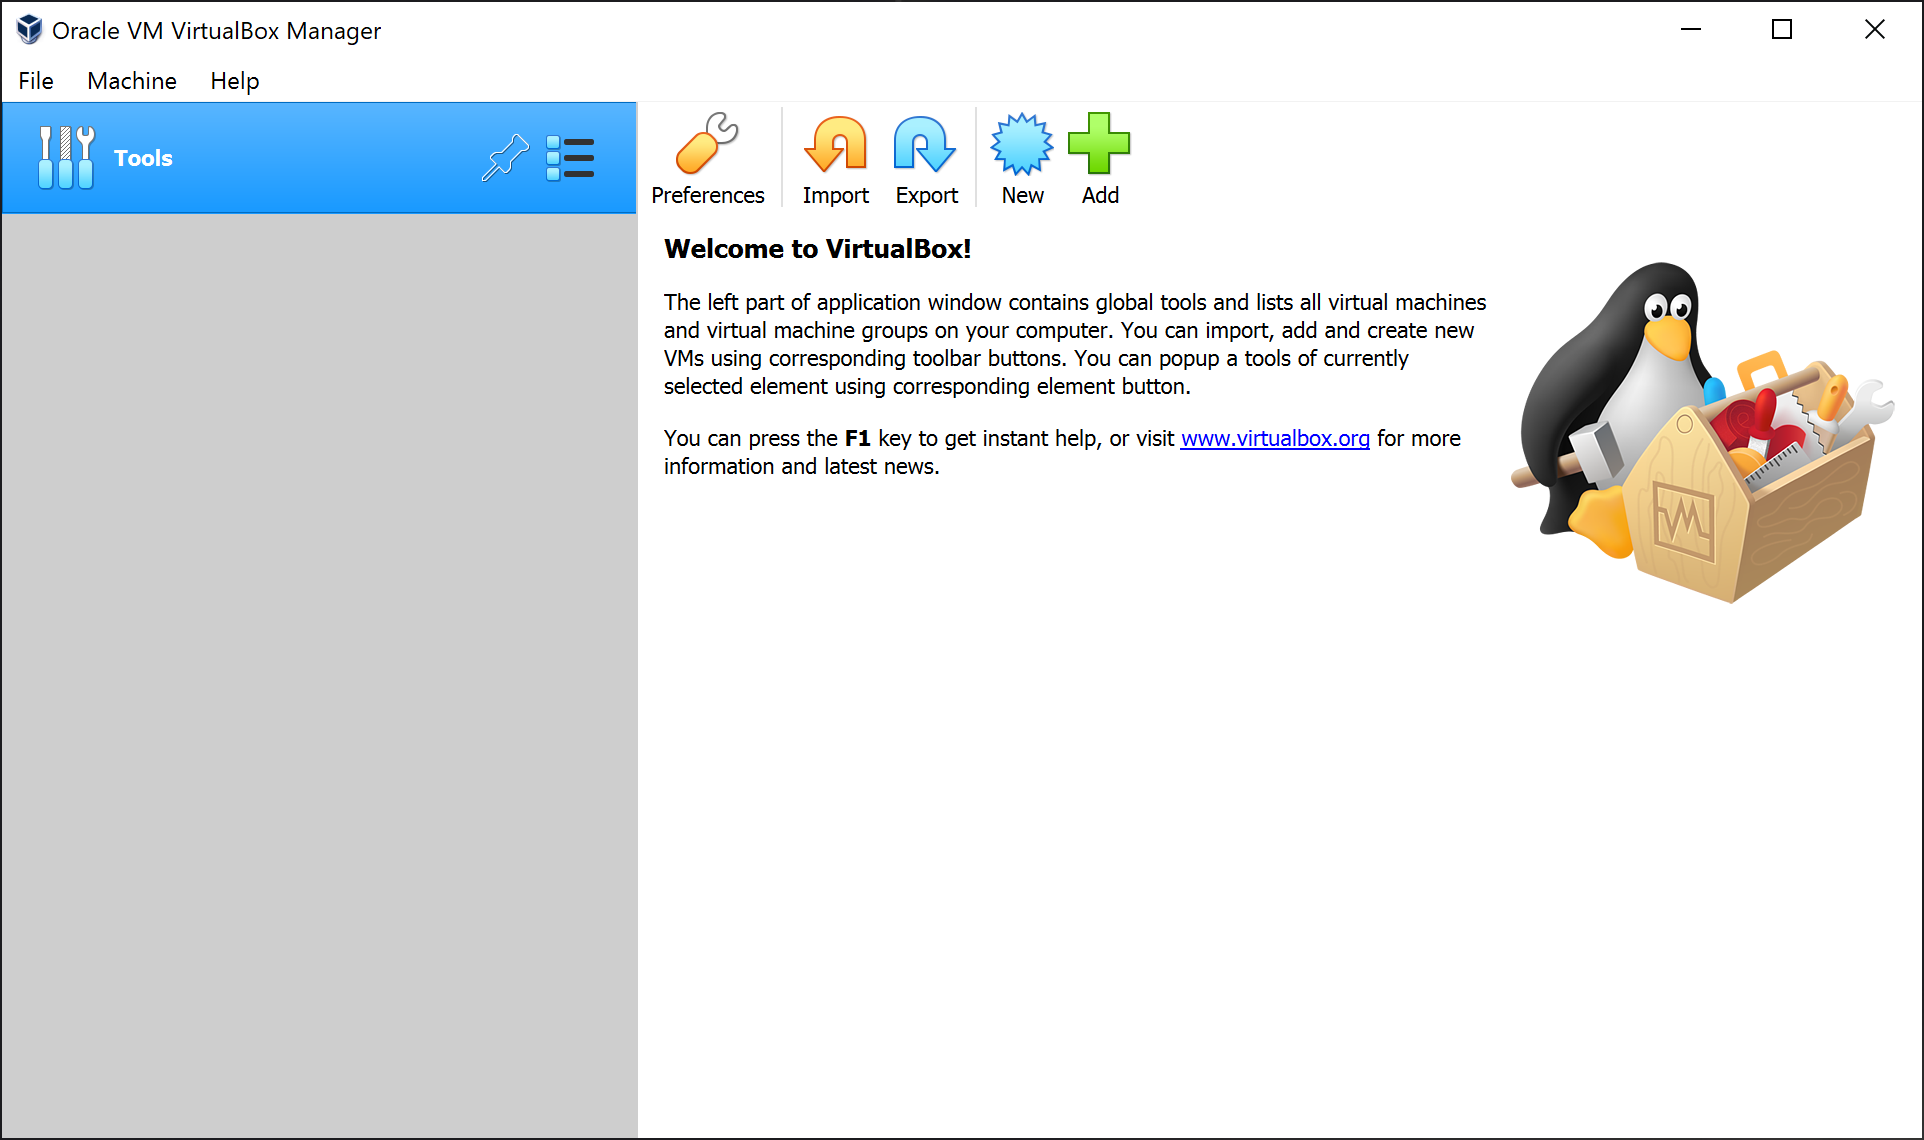
\includegraphics[width=0.7\textwidth]{ECE4310_Proj3_1_installed.png}
\end{figure}

\subsection{Download Ubuntu Server 18.10}
\begin{figure}[H]
  \caption{ISO image is downloaded}
  \centering
  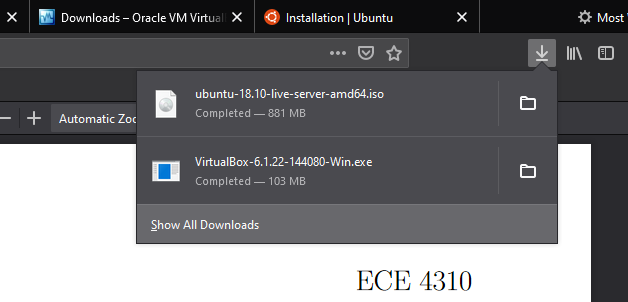
\includegraphics[width=0.7\textwidth]{ECE4310_Proj3_1_downloaded.png}
\end{figure}

\subsection{Create VM}
\begin{figure}[H]
  \caption{VM is created and configured to boot with Live CD image}
  \centering
  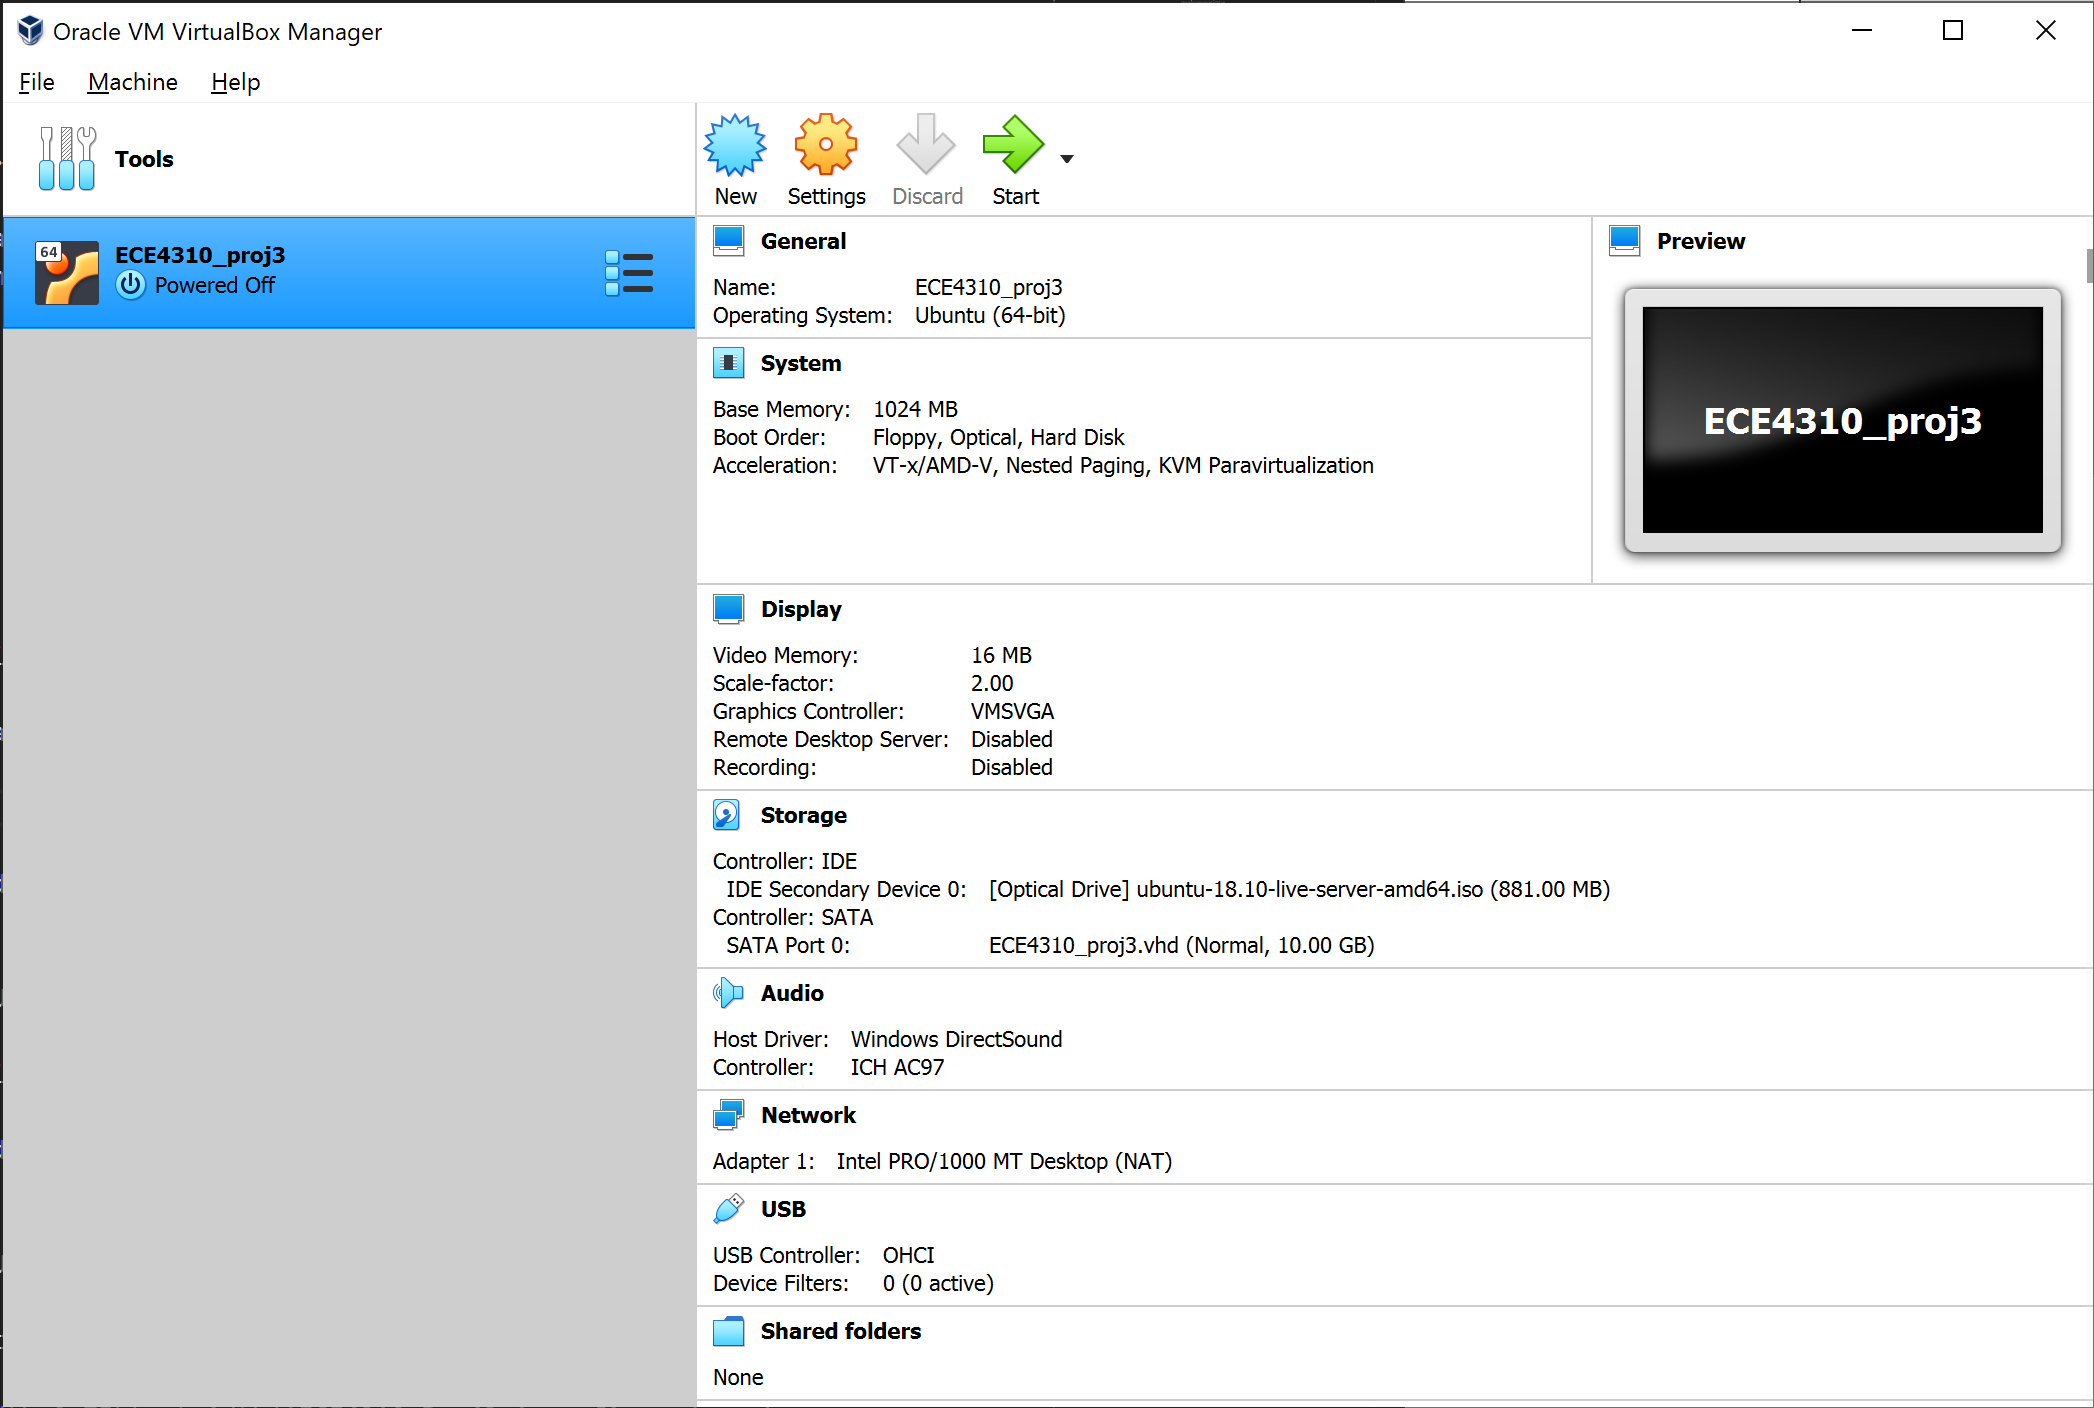
\includegraphics[width=0.7\textwidth]{ECE4310_Proj3_1_configured.png}
\end{figure}

\subsection{Install Ubuntu}
\begin{figure}[H]
  \caption{Ubuntu is being installed}
  \centering
  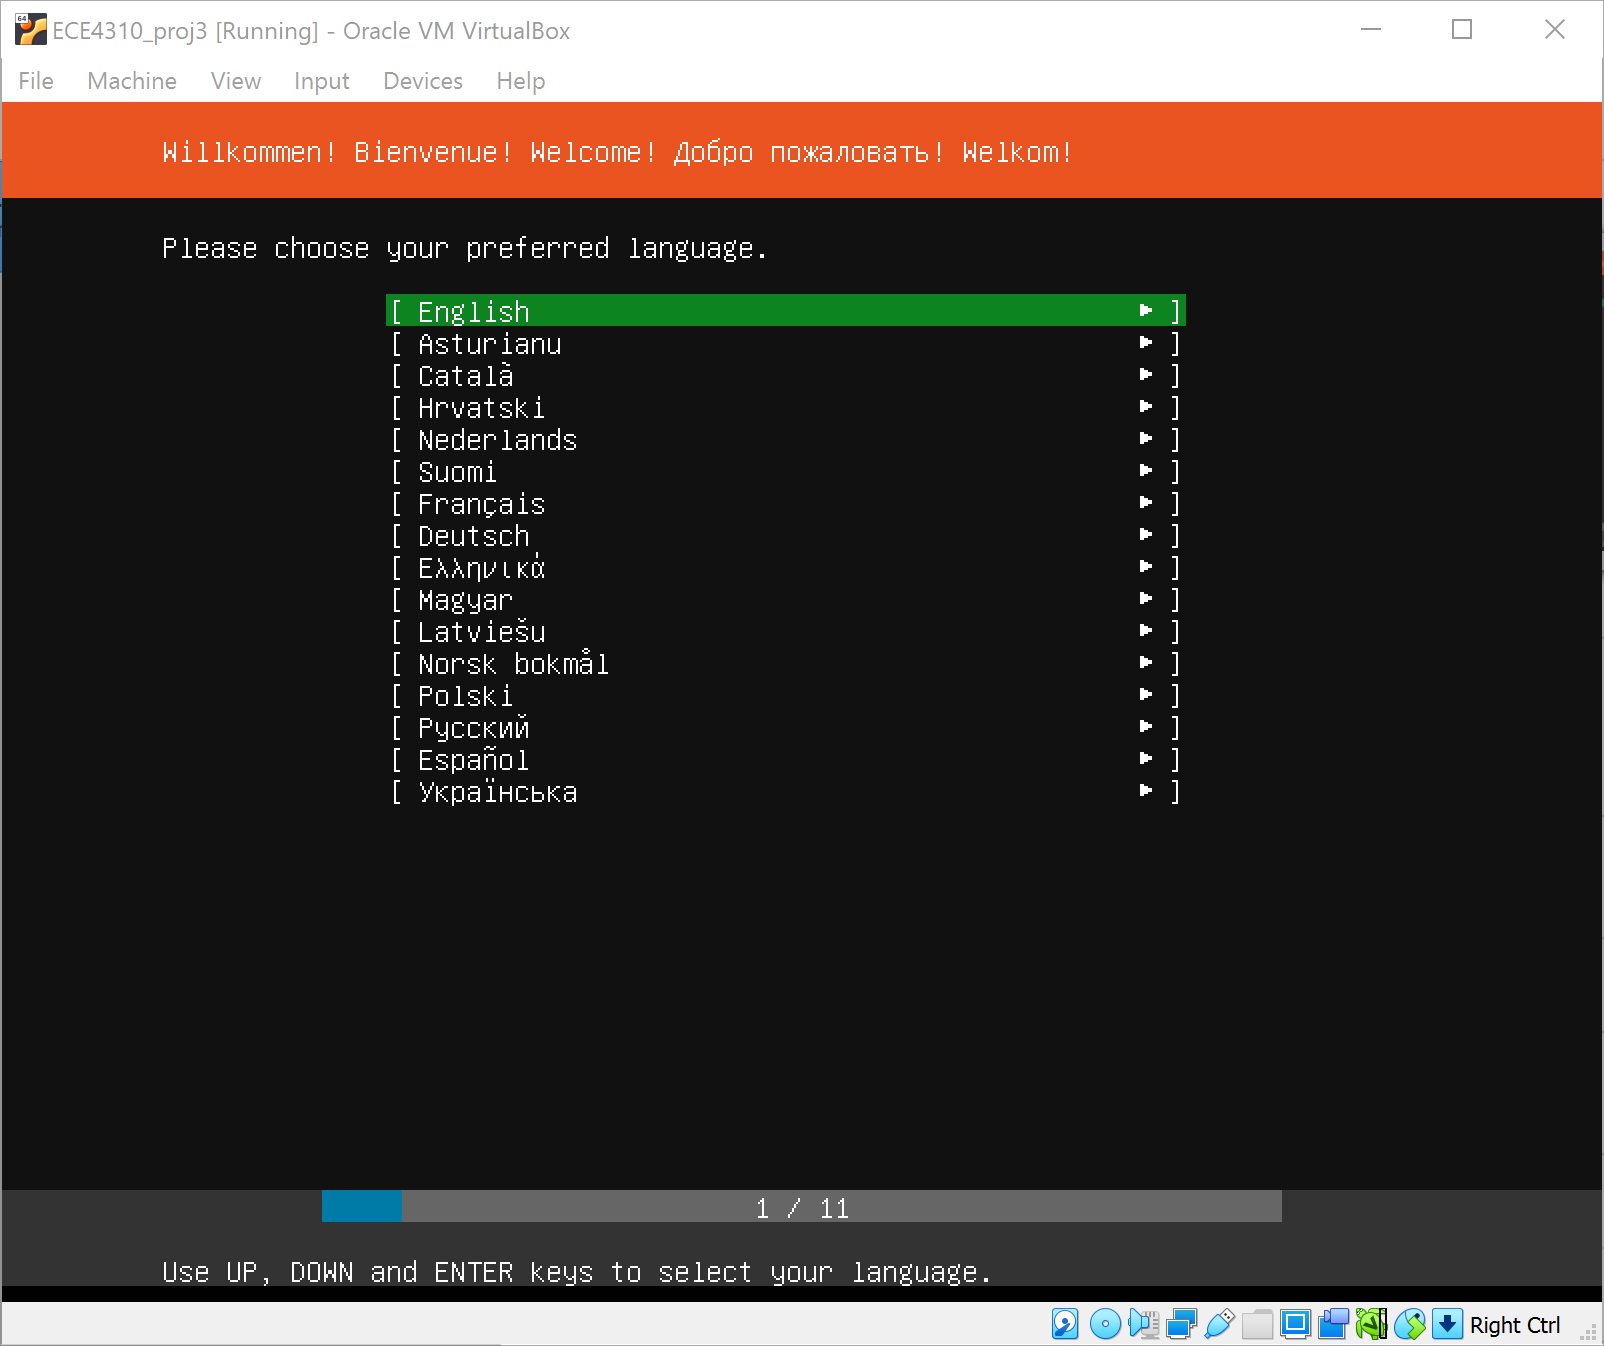
\includegraphics[width=0.7\textwidth]{ECE4310_Proj3_1_installing_1.png}
\end{figure}

\begin{figure}[H]
  \caption{Ubuntu is being installed}
  \centering
  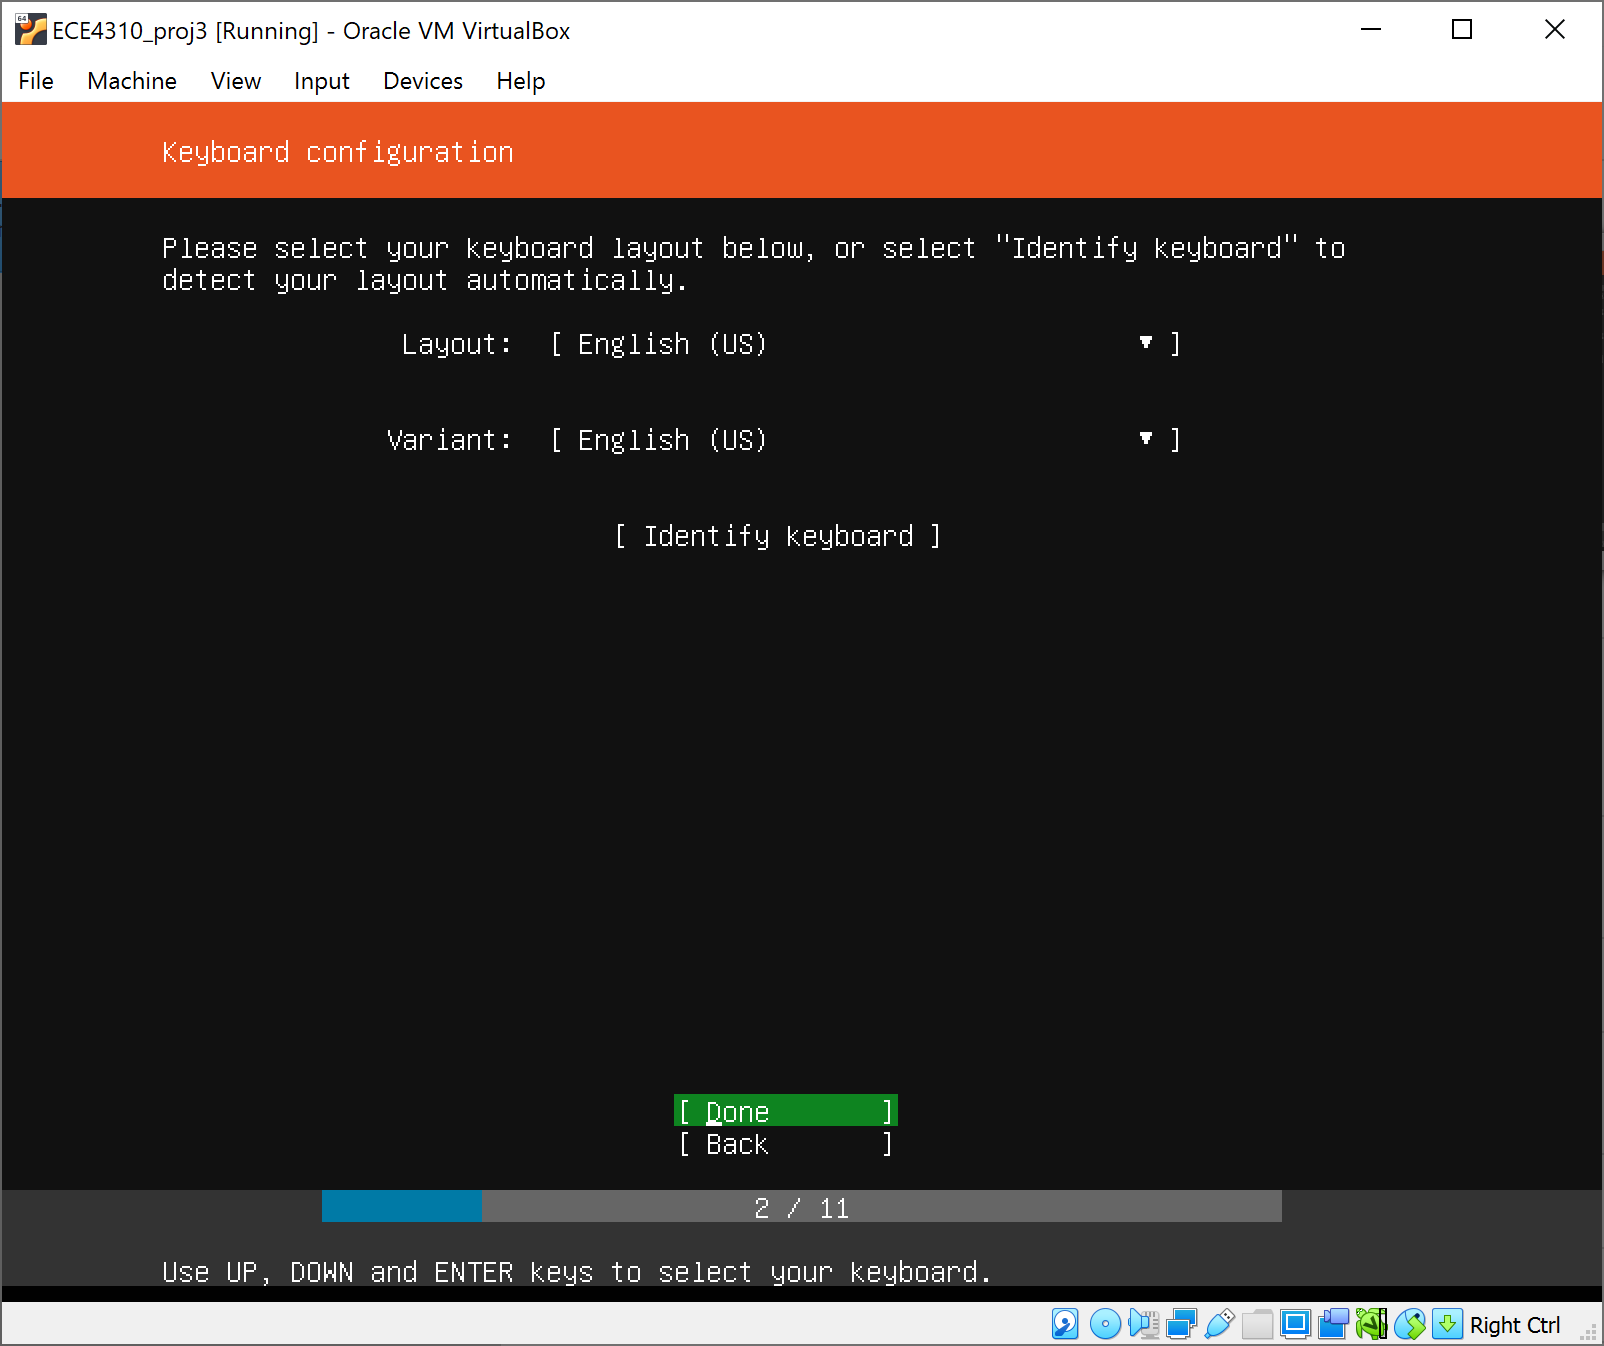
\includegraphics[width=0.7\textwidth]{ECE4310_Proj3_1_installing_2.png}
\end{figure}

\begin{figure}[H]
  \caption{Ubuntu is being installed}
  \centering
  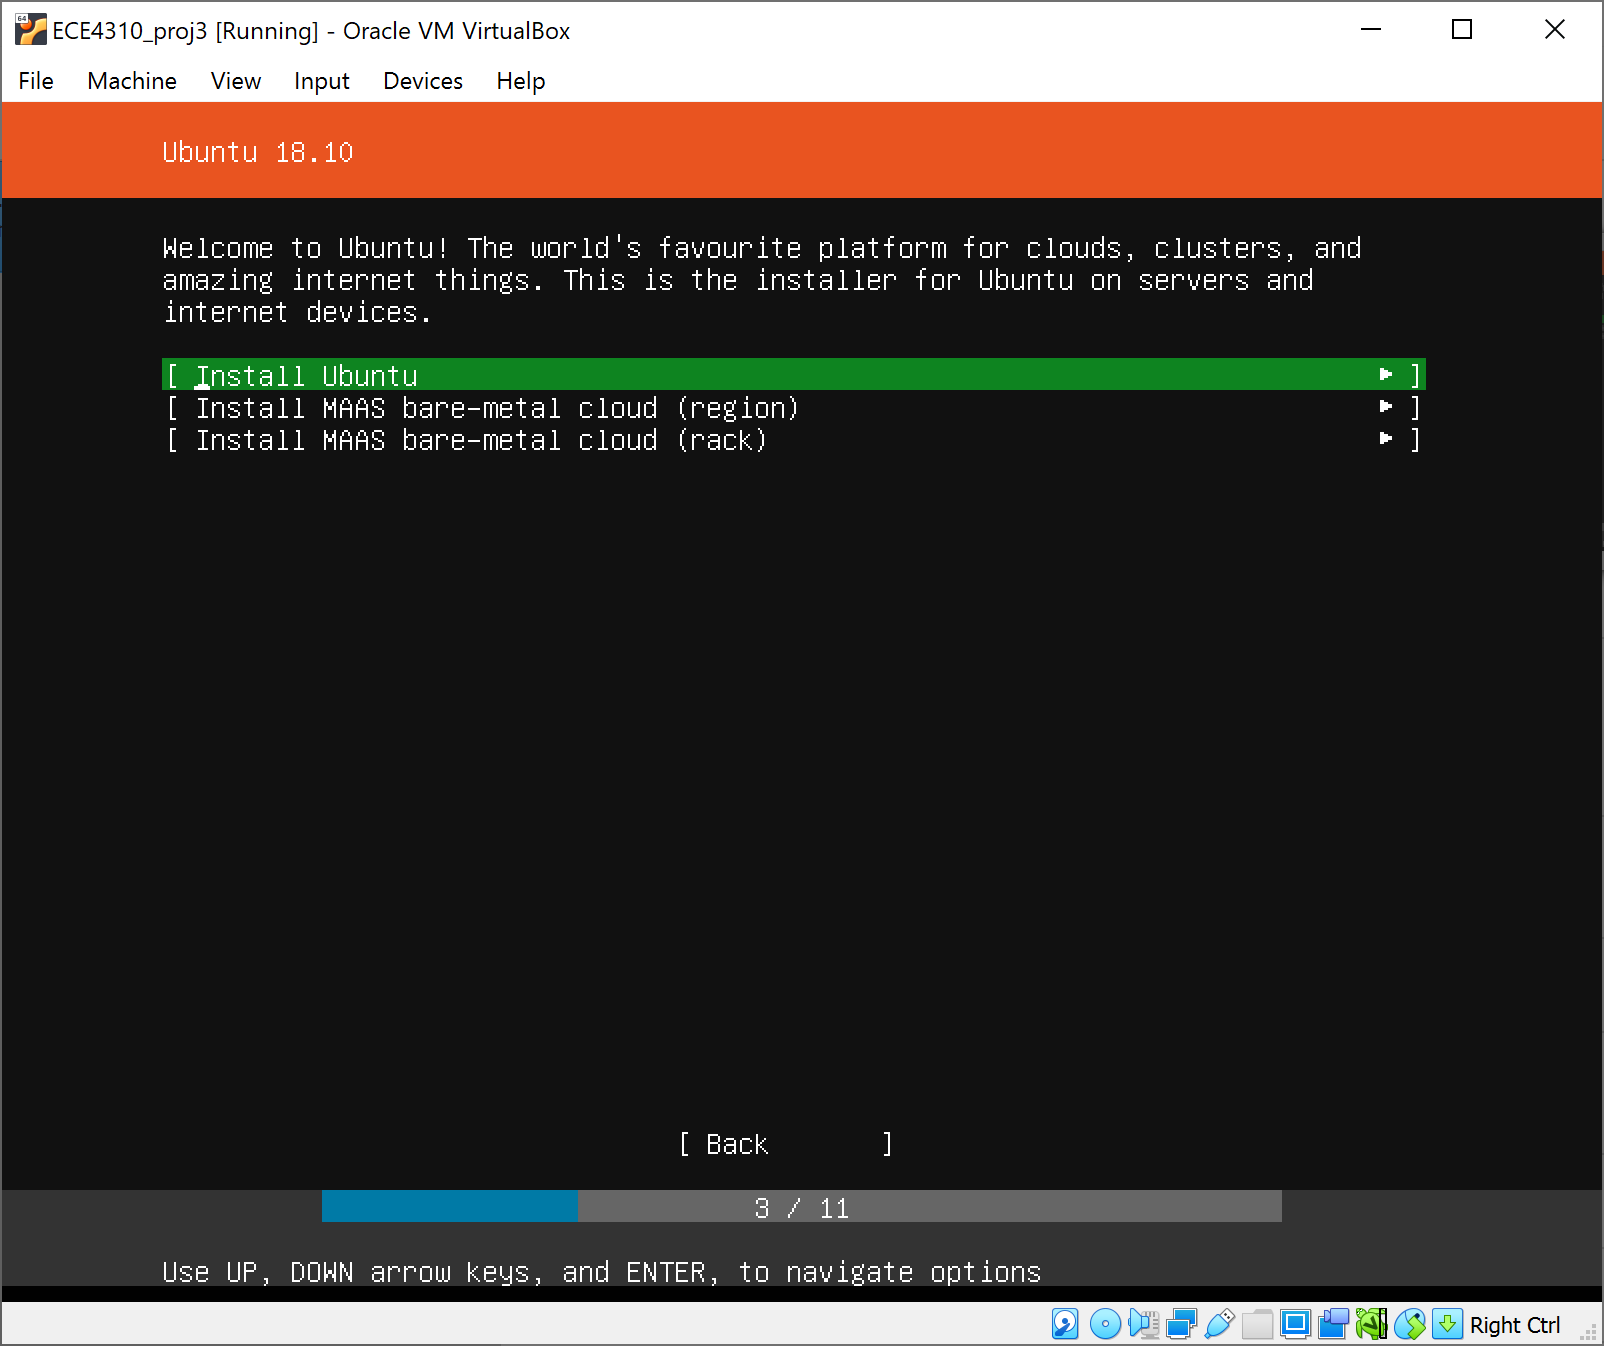
\includegraphics[width=0.7\textwidth]{ECE4310_Proj3_1_installing_3.png}
\end{figure}

\begin{figure}[H]
  \caption{Ubuntu is being installed}
  \centering
  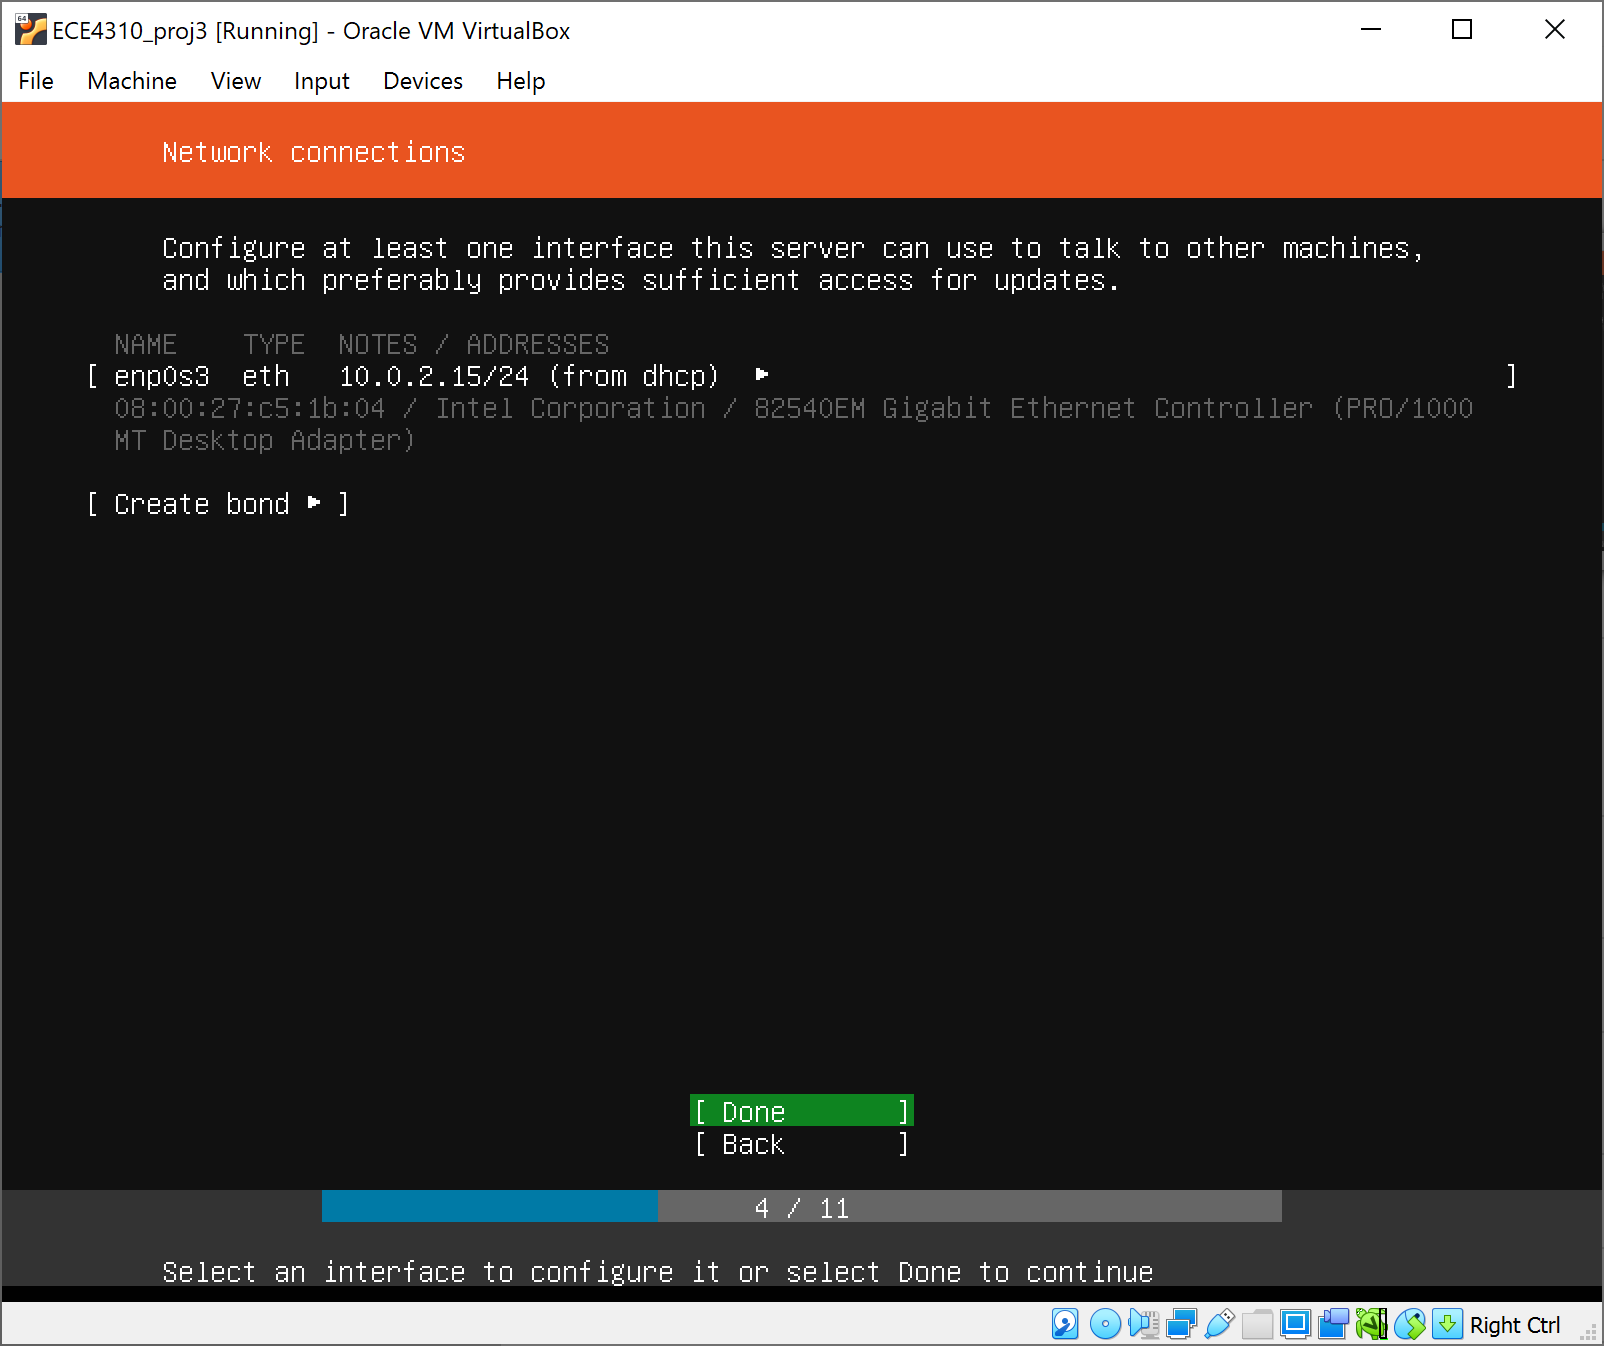
\includegraphics[width=0.7\textwidth]{ECE4310_Proj3_1_installing_4.png}
\end{figure}

\begin{figure}[H]
  \caption{Ubuntu is being installed}
  \centering
  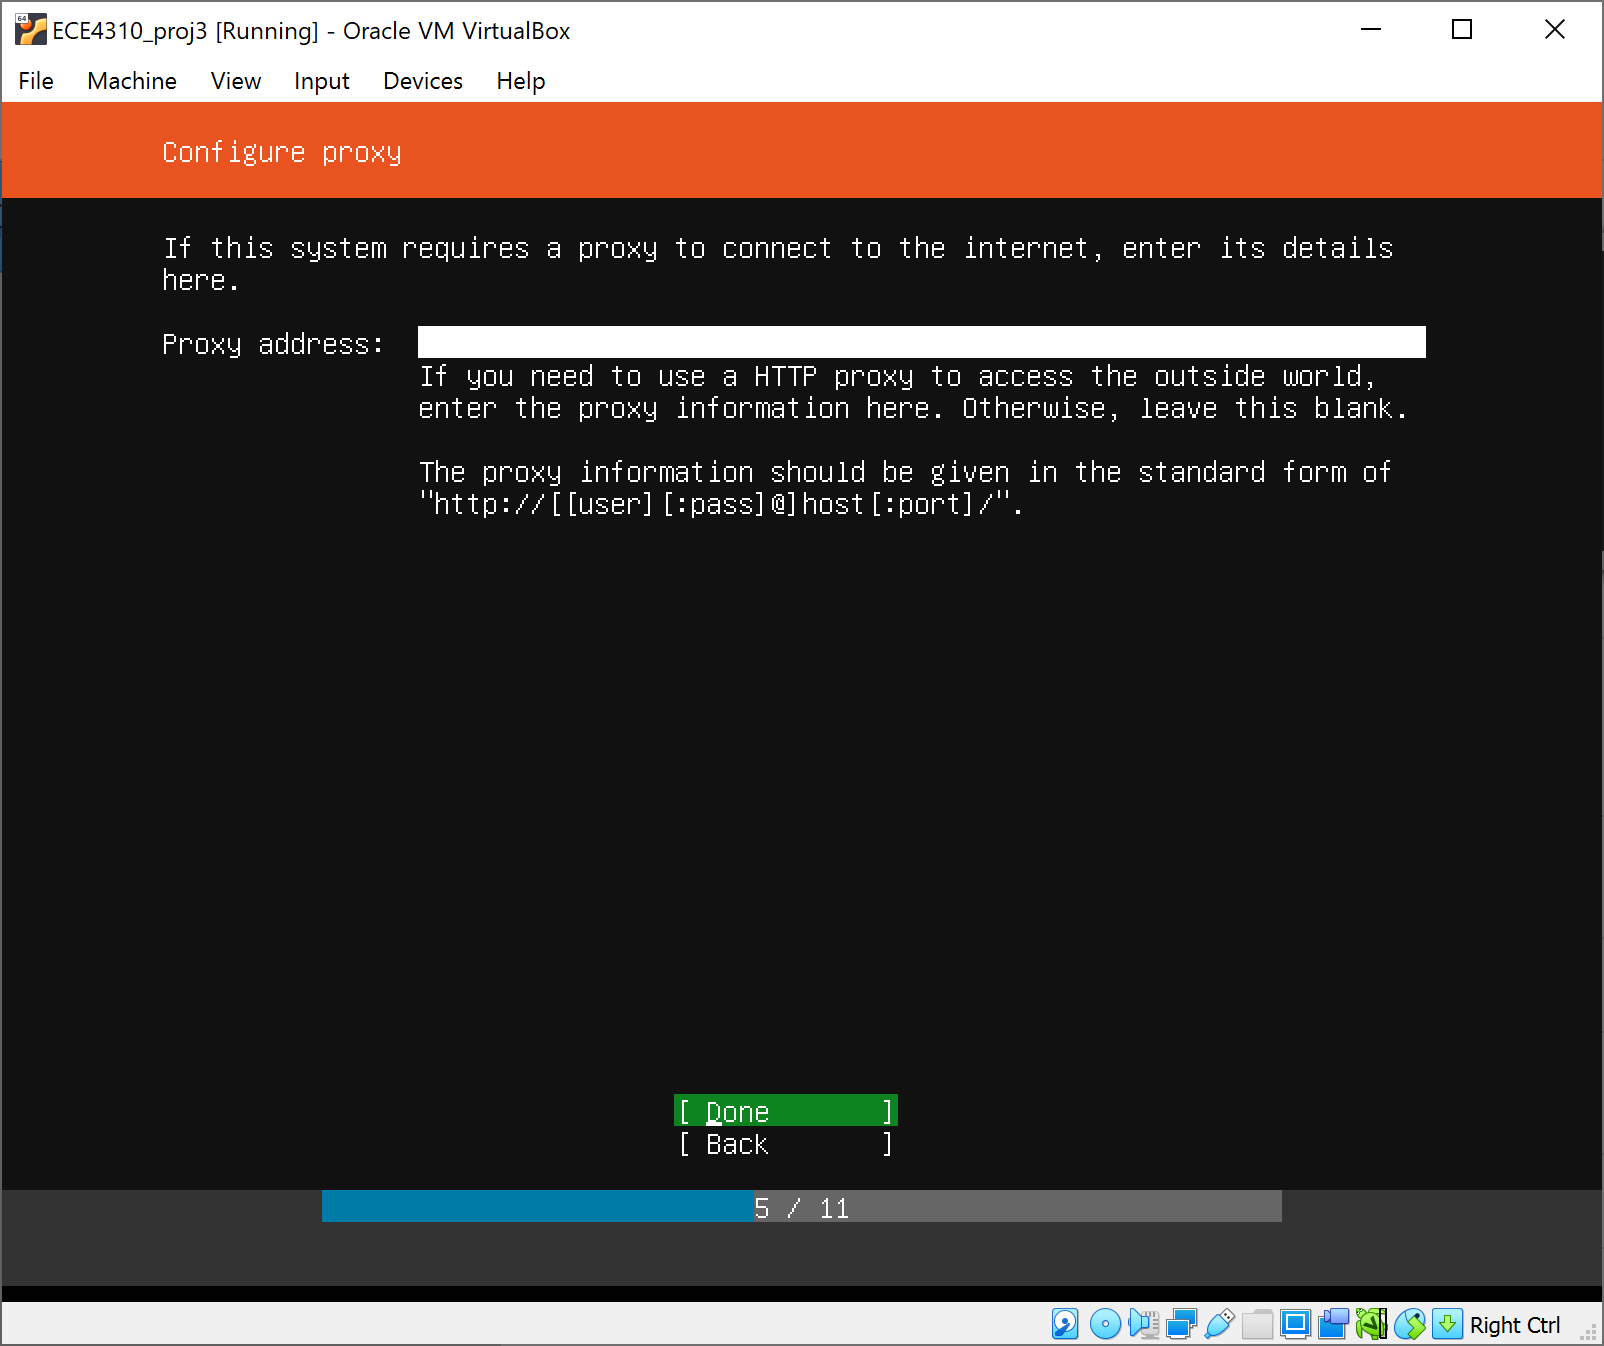
\includegraphics[width=0.7\textwidth]{ECE4310_Proj3_1_installing_5.png}
\end{figure}

\begin{figure}[H]
  \caption{Ubuntu is being installed}
  \centering
  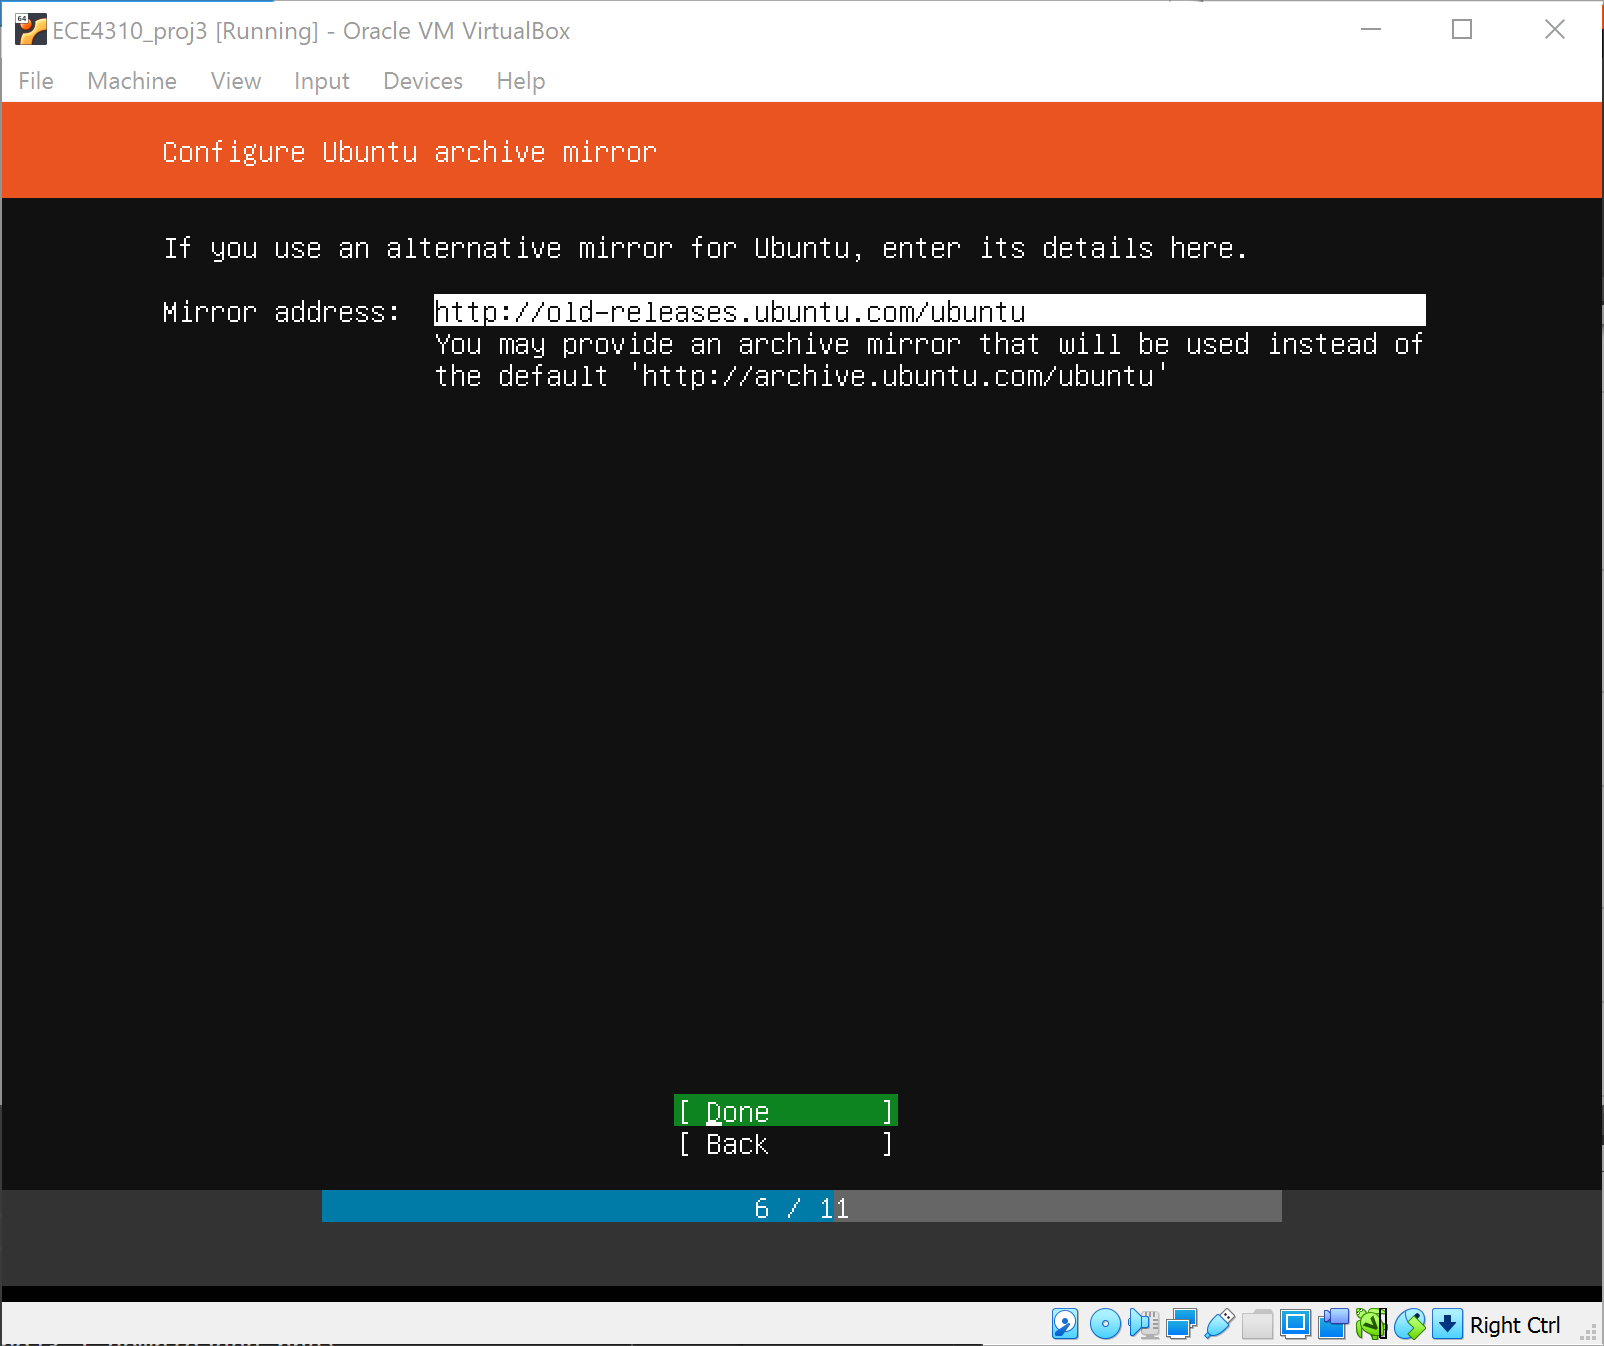
\includegraphics[width=0.7\textwidth]{ECE4310_Proj3_1_installing_6.png}
\end{figure}

\begin{figure}[H]
  \caption{Ubuntu is being installed}
  \centering
  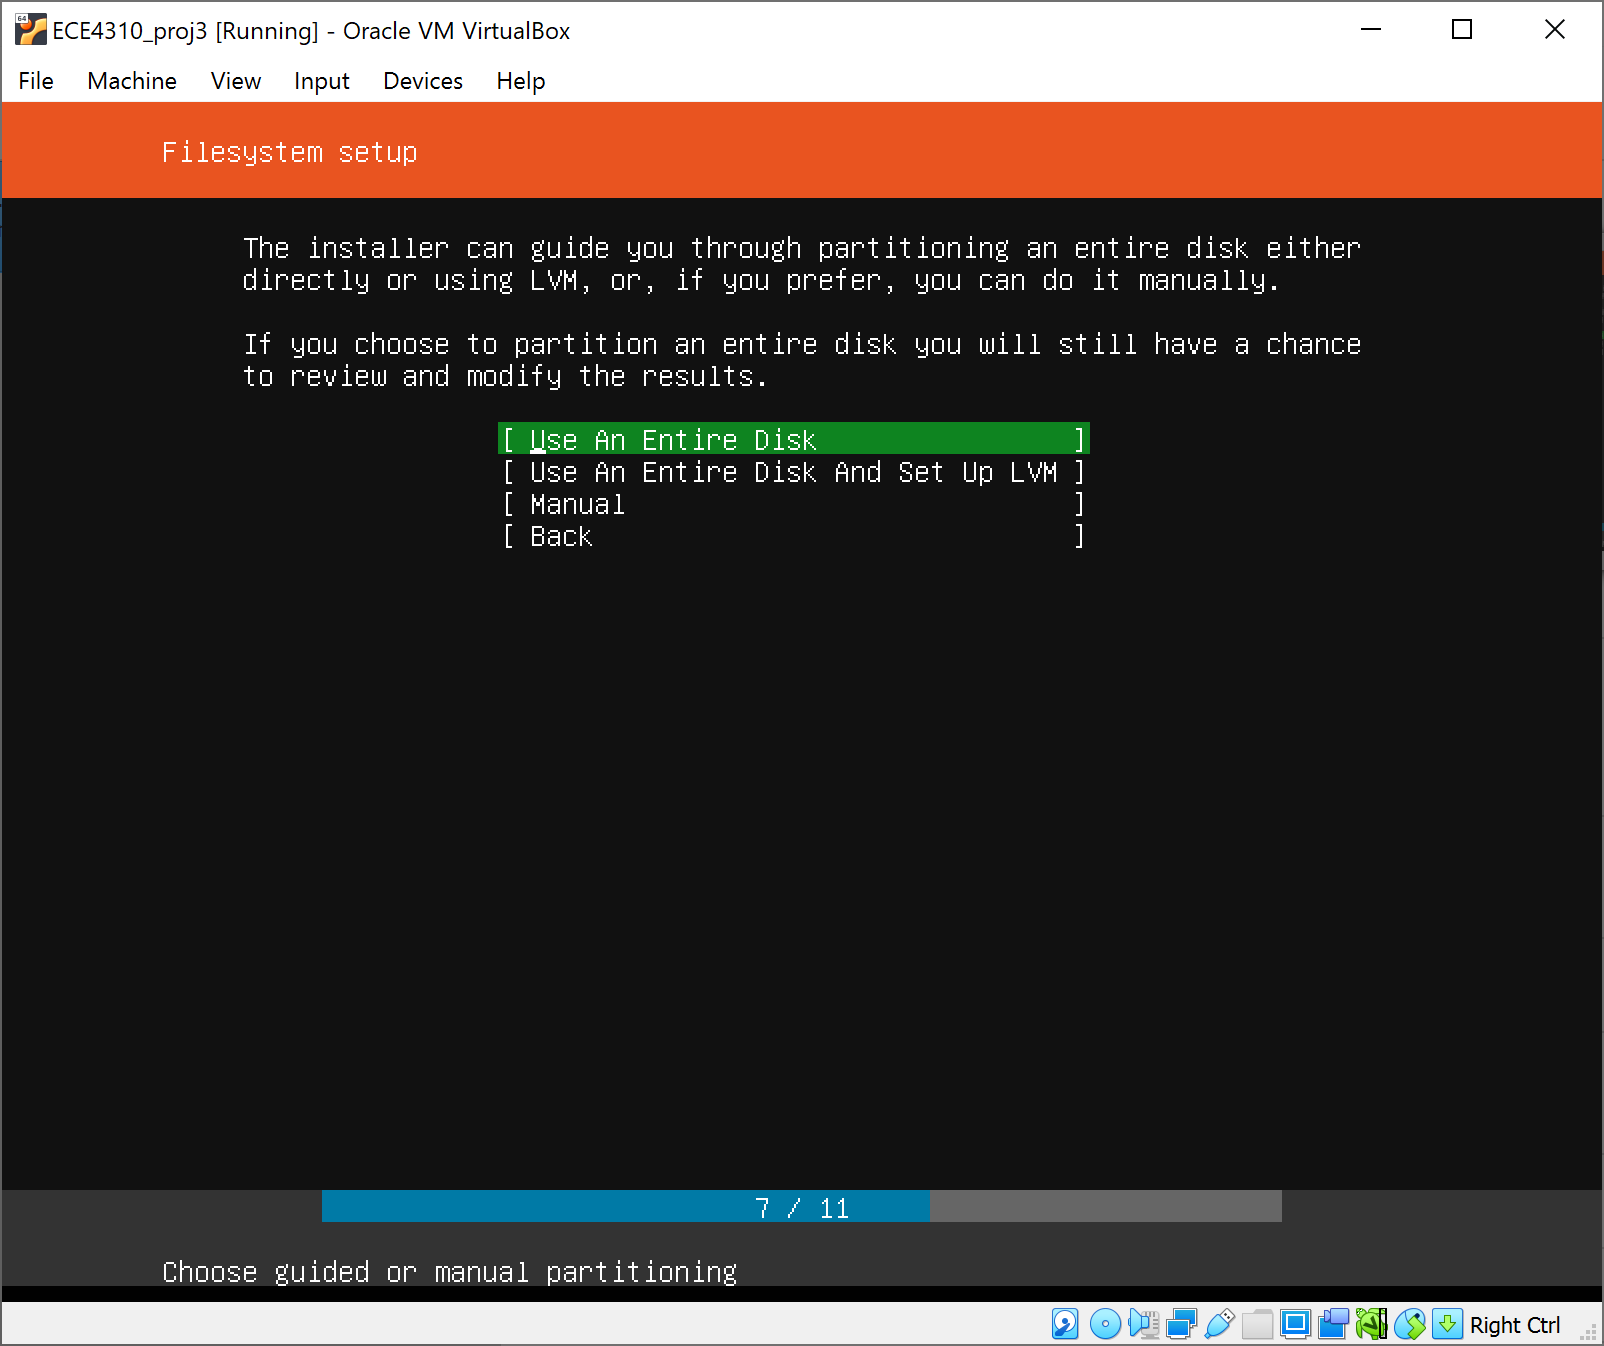
\includegraphics[width=0.7\textwidth]{ECE4310_Proj3_1_installing_7.png}
\end{figure}

\begin{figure}[H]
  \caption{Ubuntu is being installed}
  \centering
  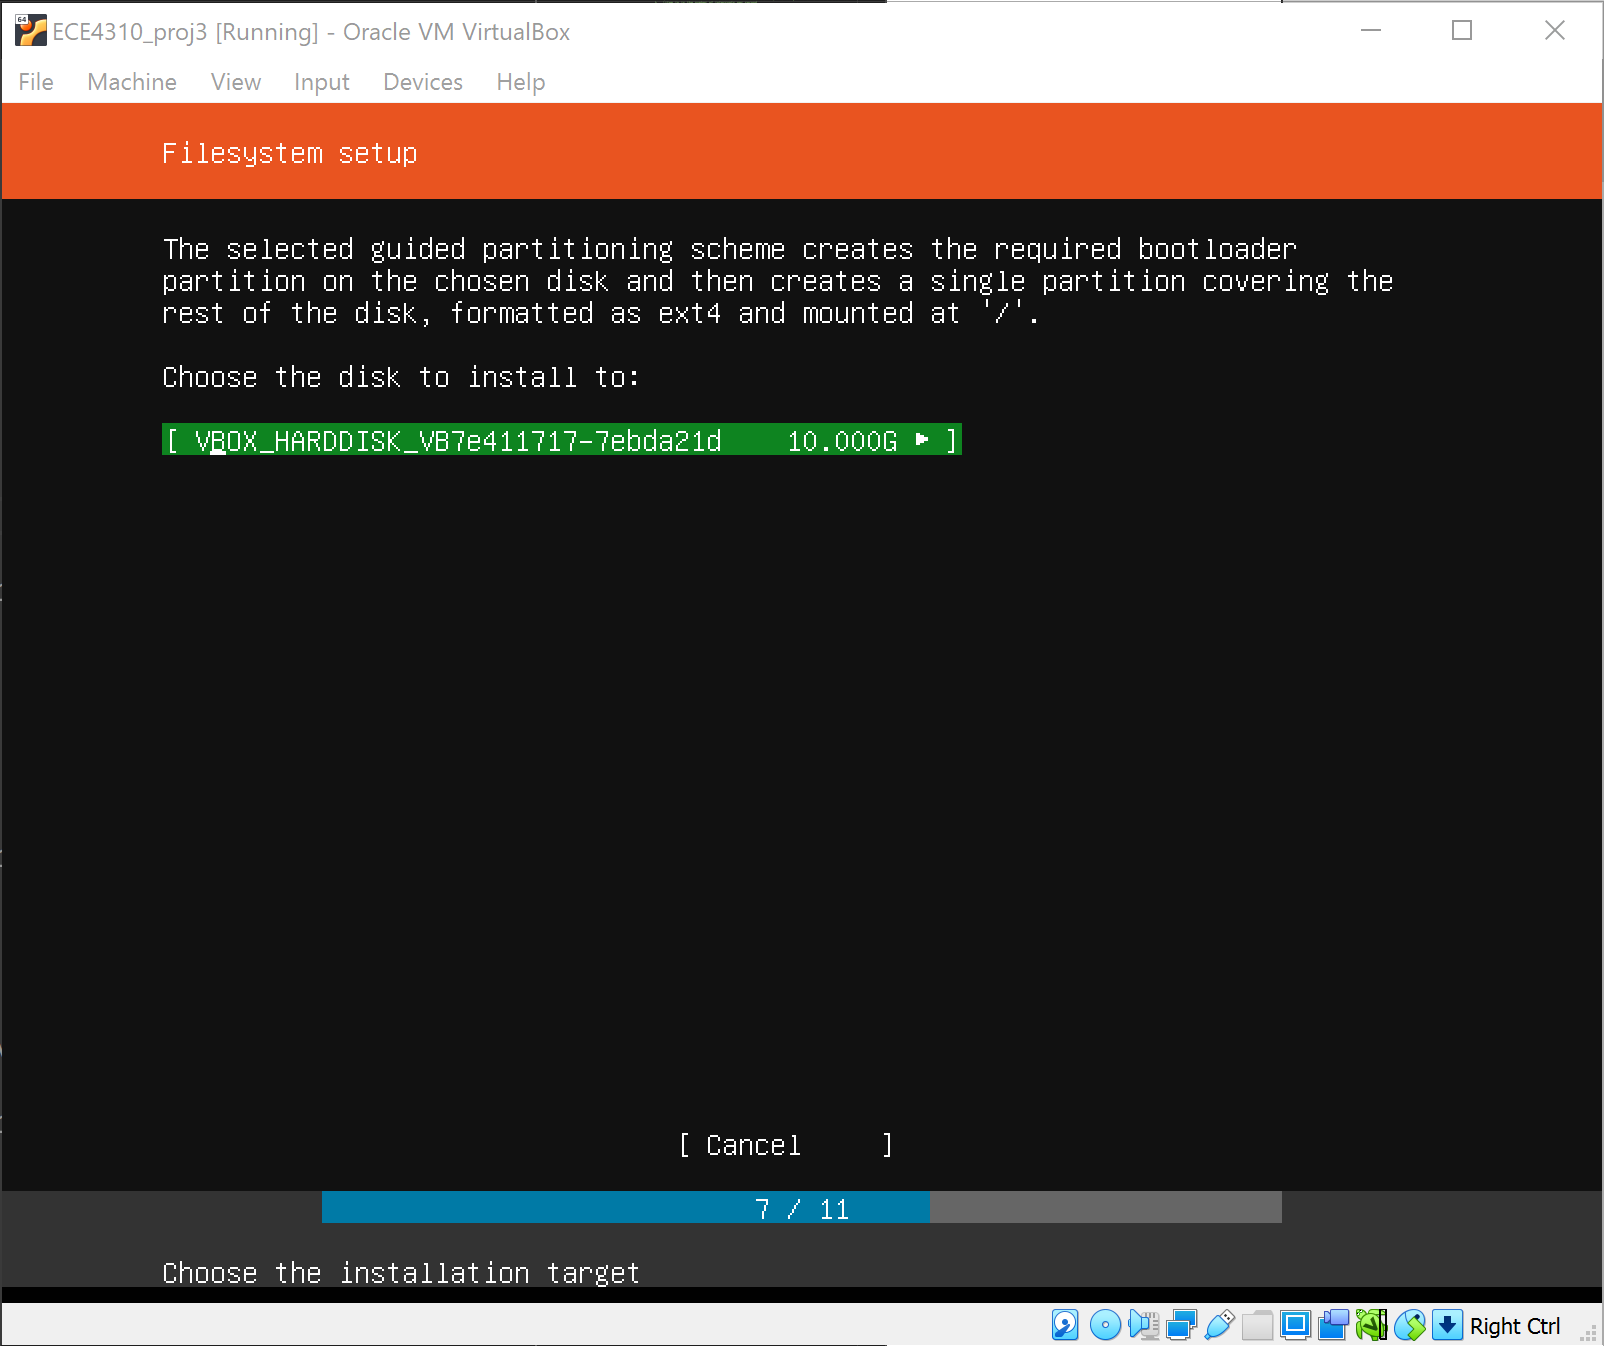
\includegraphics[width=0.7\textwidth]{ECE4310_Proj3_1_installing_7_2.png}
\end{figure}

\begin{figure}[H]
  \caption{Ubuntu is being installed}
  \centering
  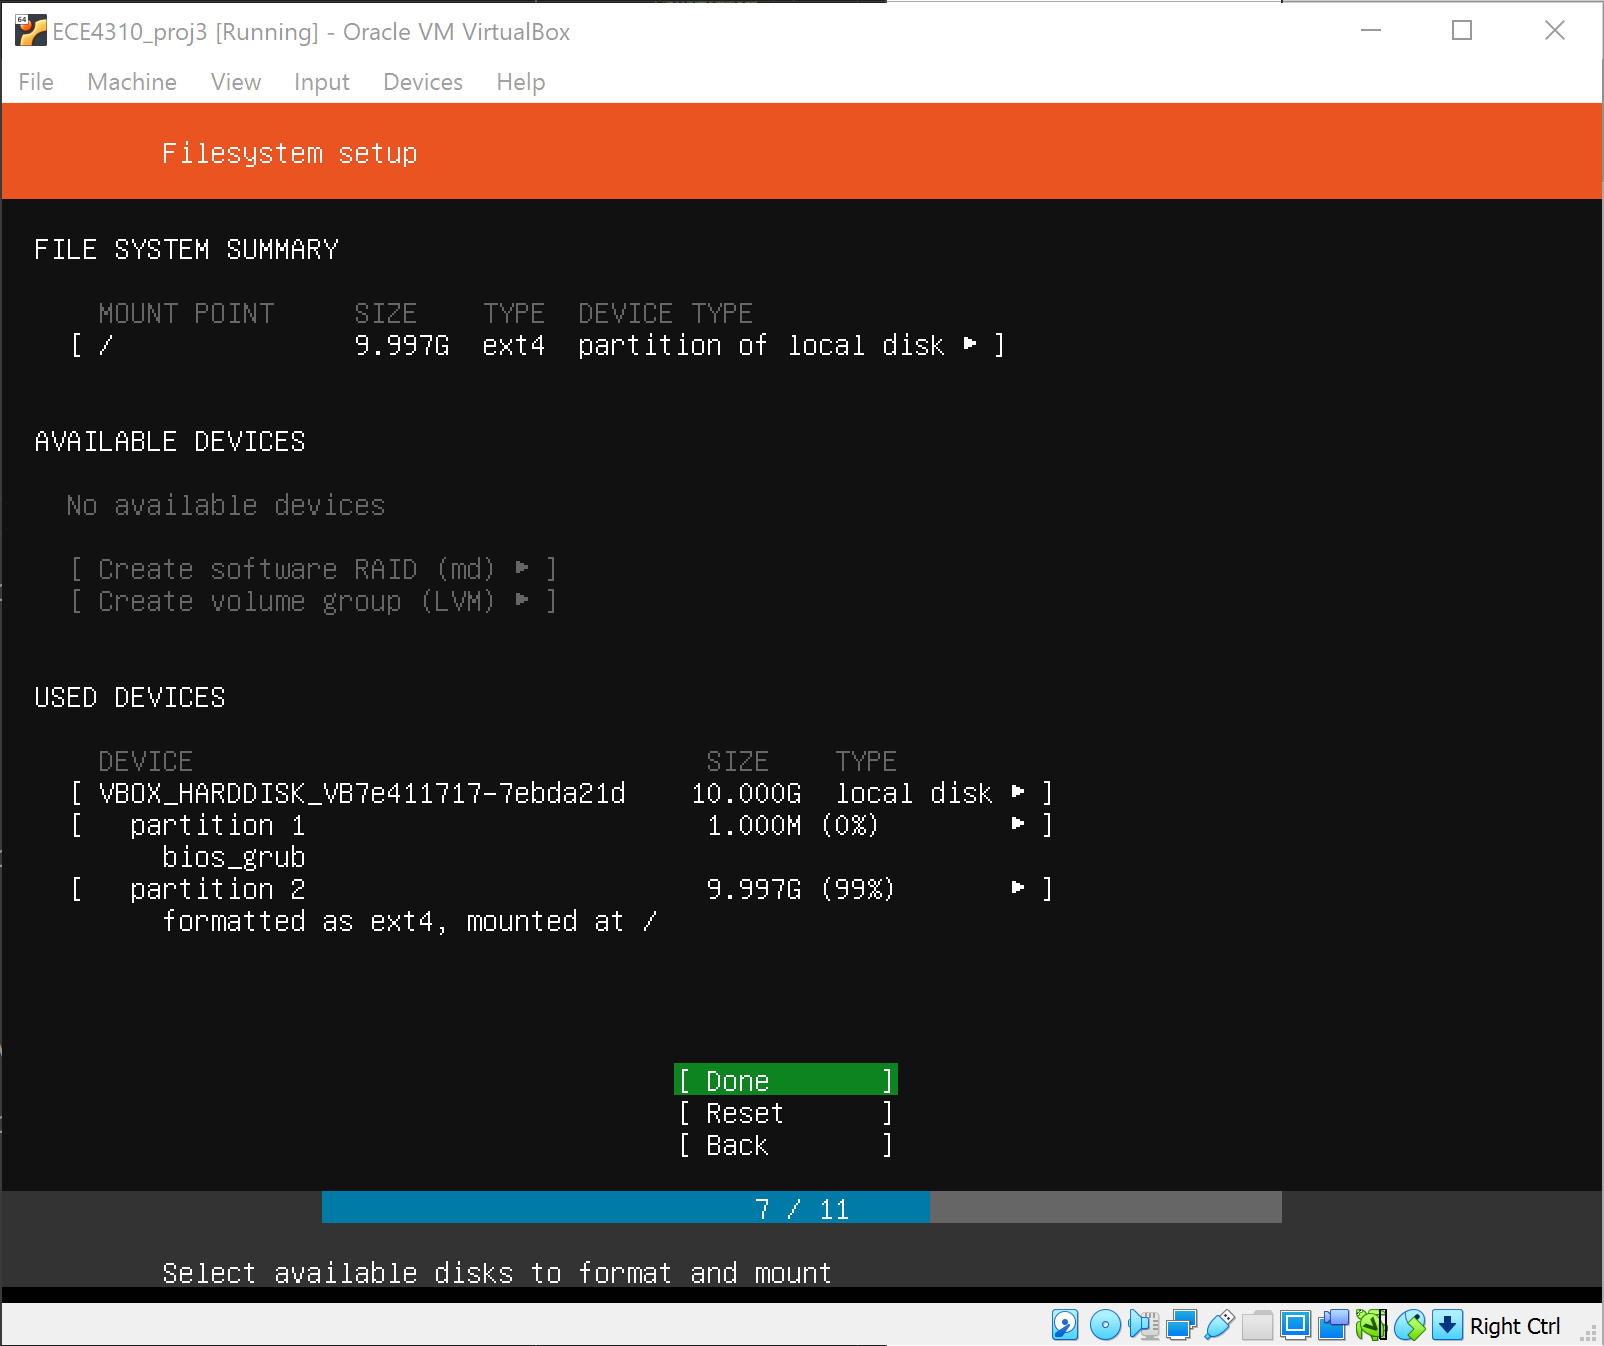
\includegraphics[width=0.7\textwidth]{ECE4310_Proj3_1_installing_7_3.png}
\end{figure}

\begin{figure}[H]
  \caption{Ubuntu is being installed}
  \centering
  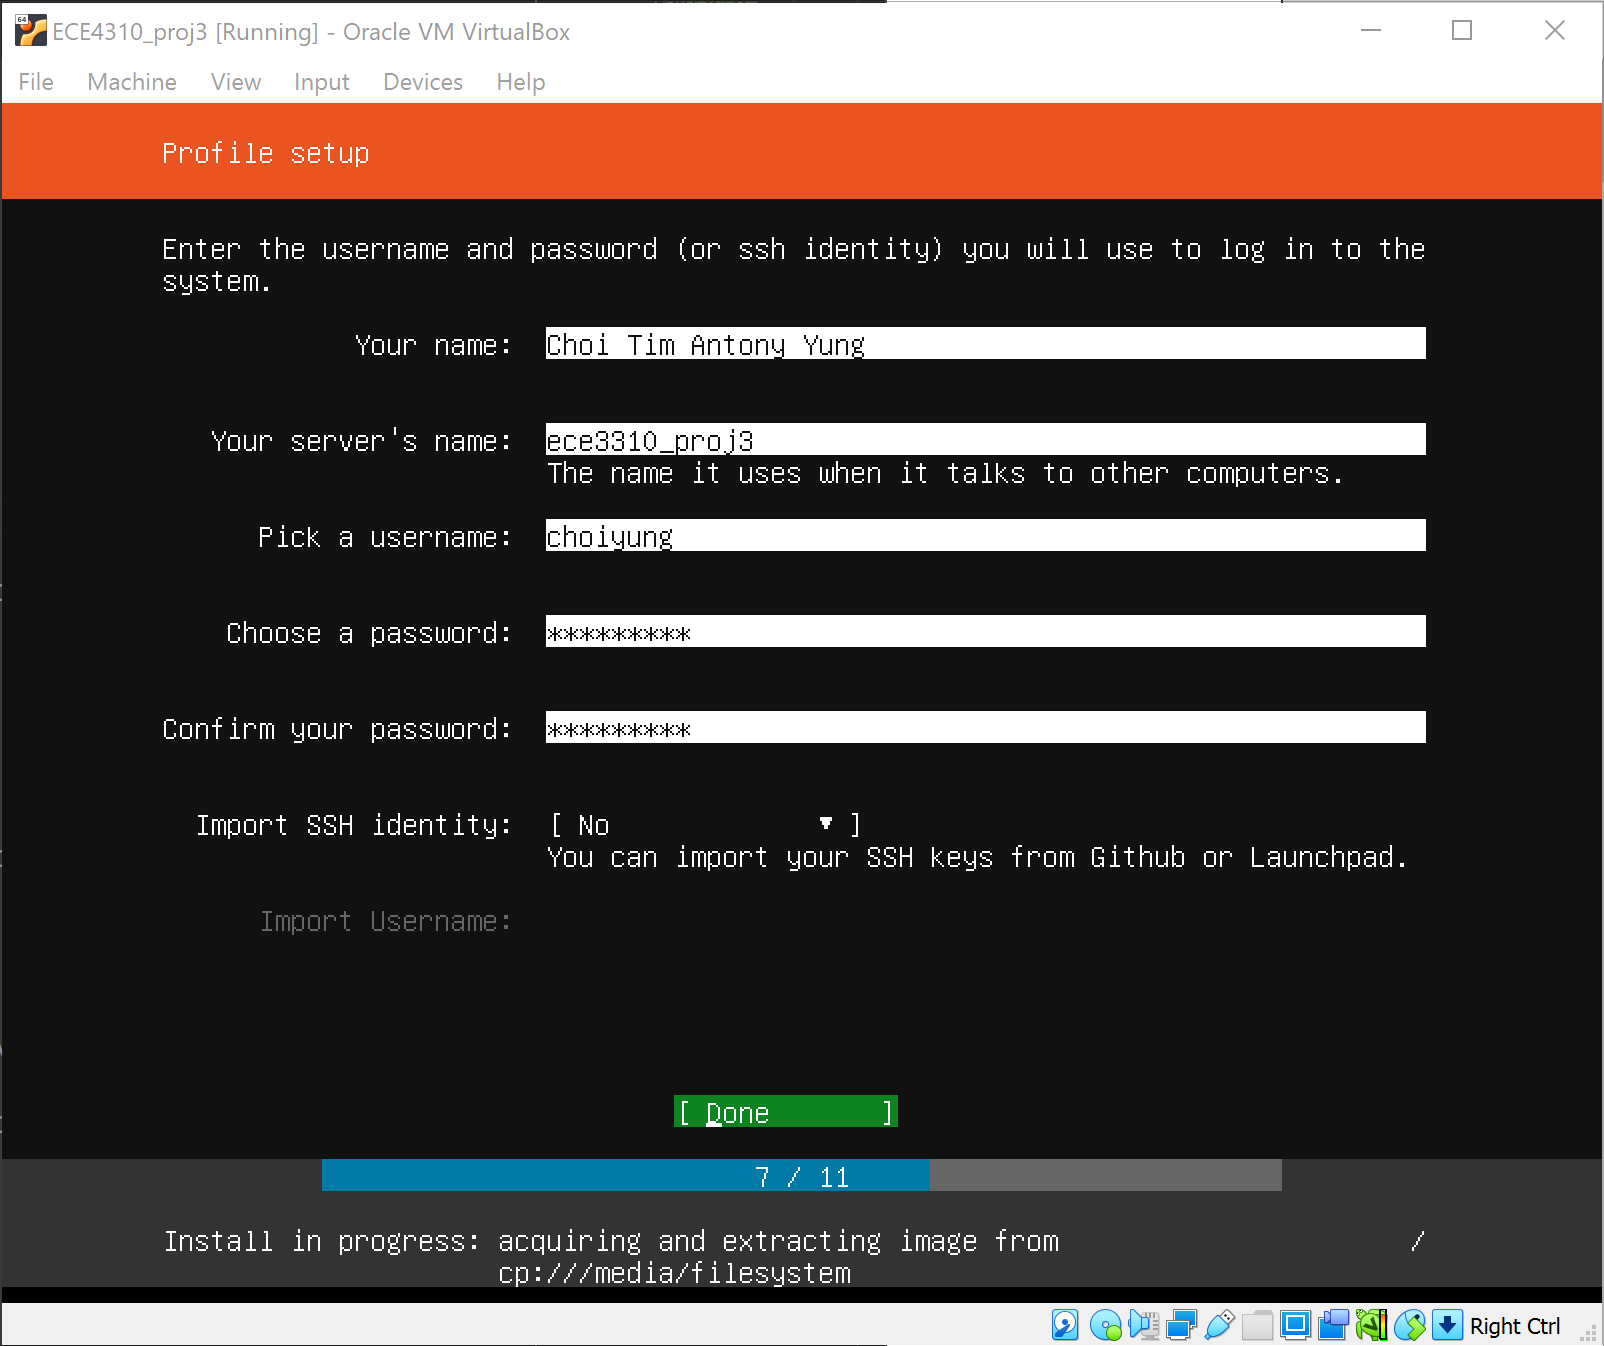
\includegraphics[width=0.7\textwidth]{ECE4310_Proj3_1_installing_7_4.png}
\end{figure}

\begin{figure}[H]
  \caption{Ubuntu is being installed}
  \centering
  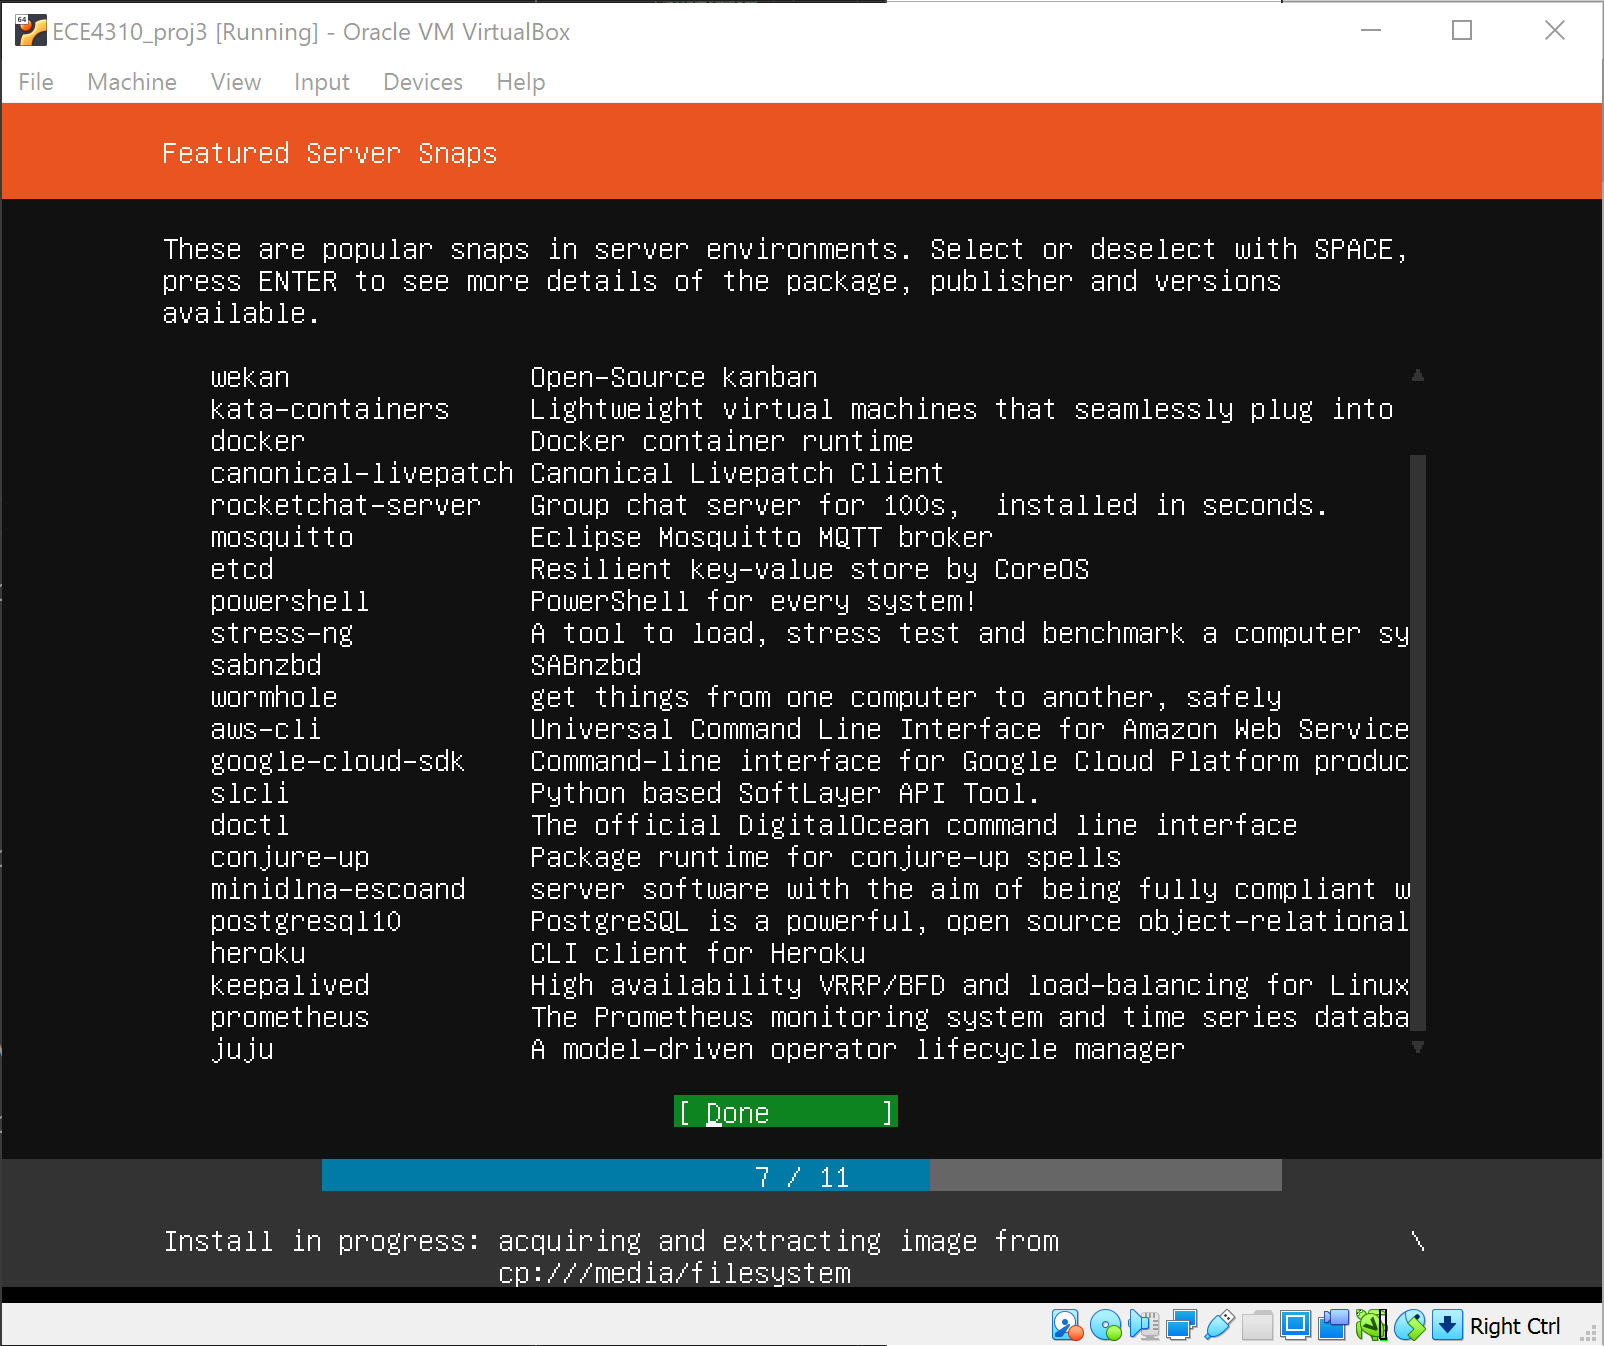
\includegraphics[width=0.7\textwidth]{ECE4310_Proj3_1_installing_7_5.png}
\end{figure}

\begin{figure}[H]
  \caption{Ubuntu is installed}
  \centering
  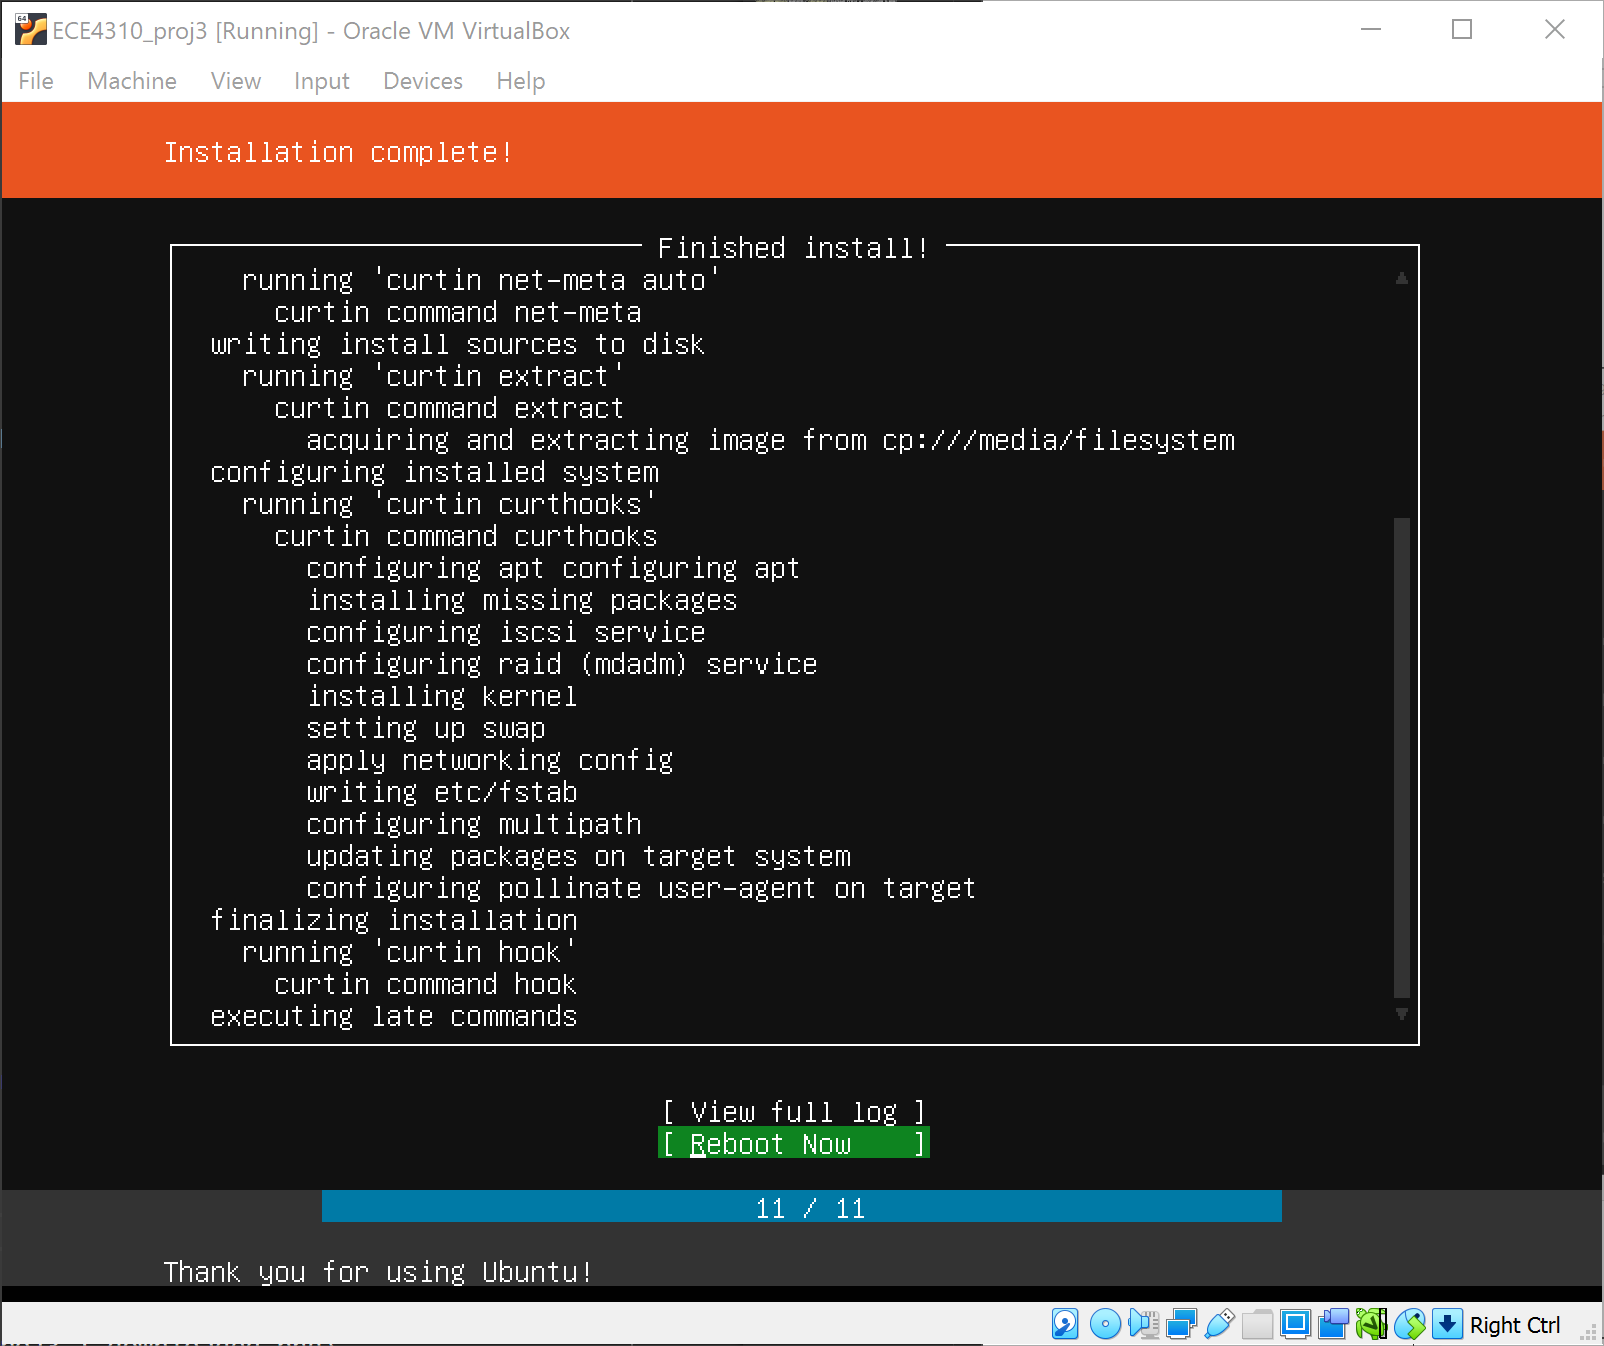
\includegraphics[width=0.7\textwidth]{ECE4310_Proj3_1_installing_11.png}
\end{figure}

\subsection{Reboot and Log in}
\begin{figure}[H]
  \caption{Successfully logged in}
  \centering
  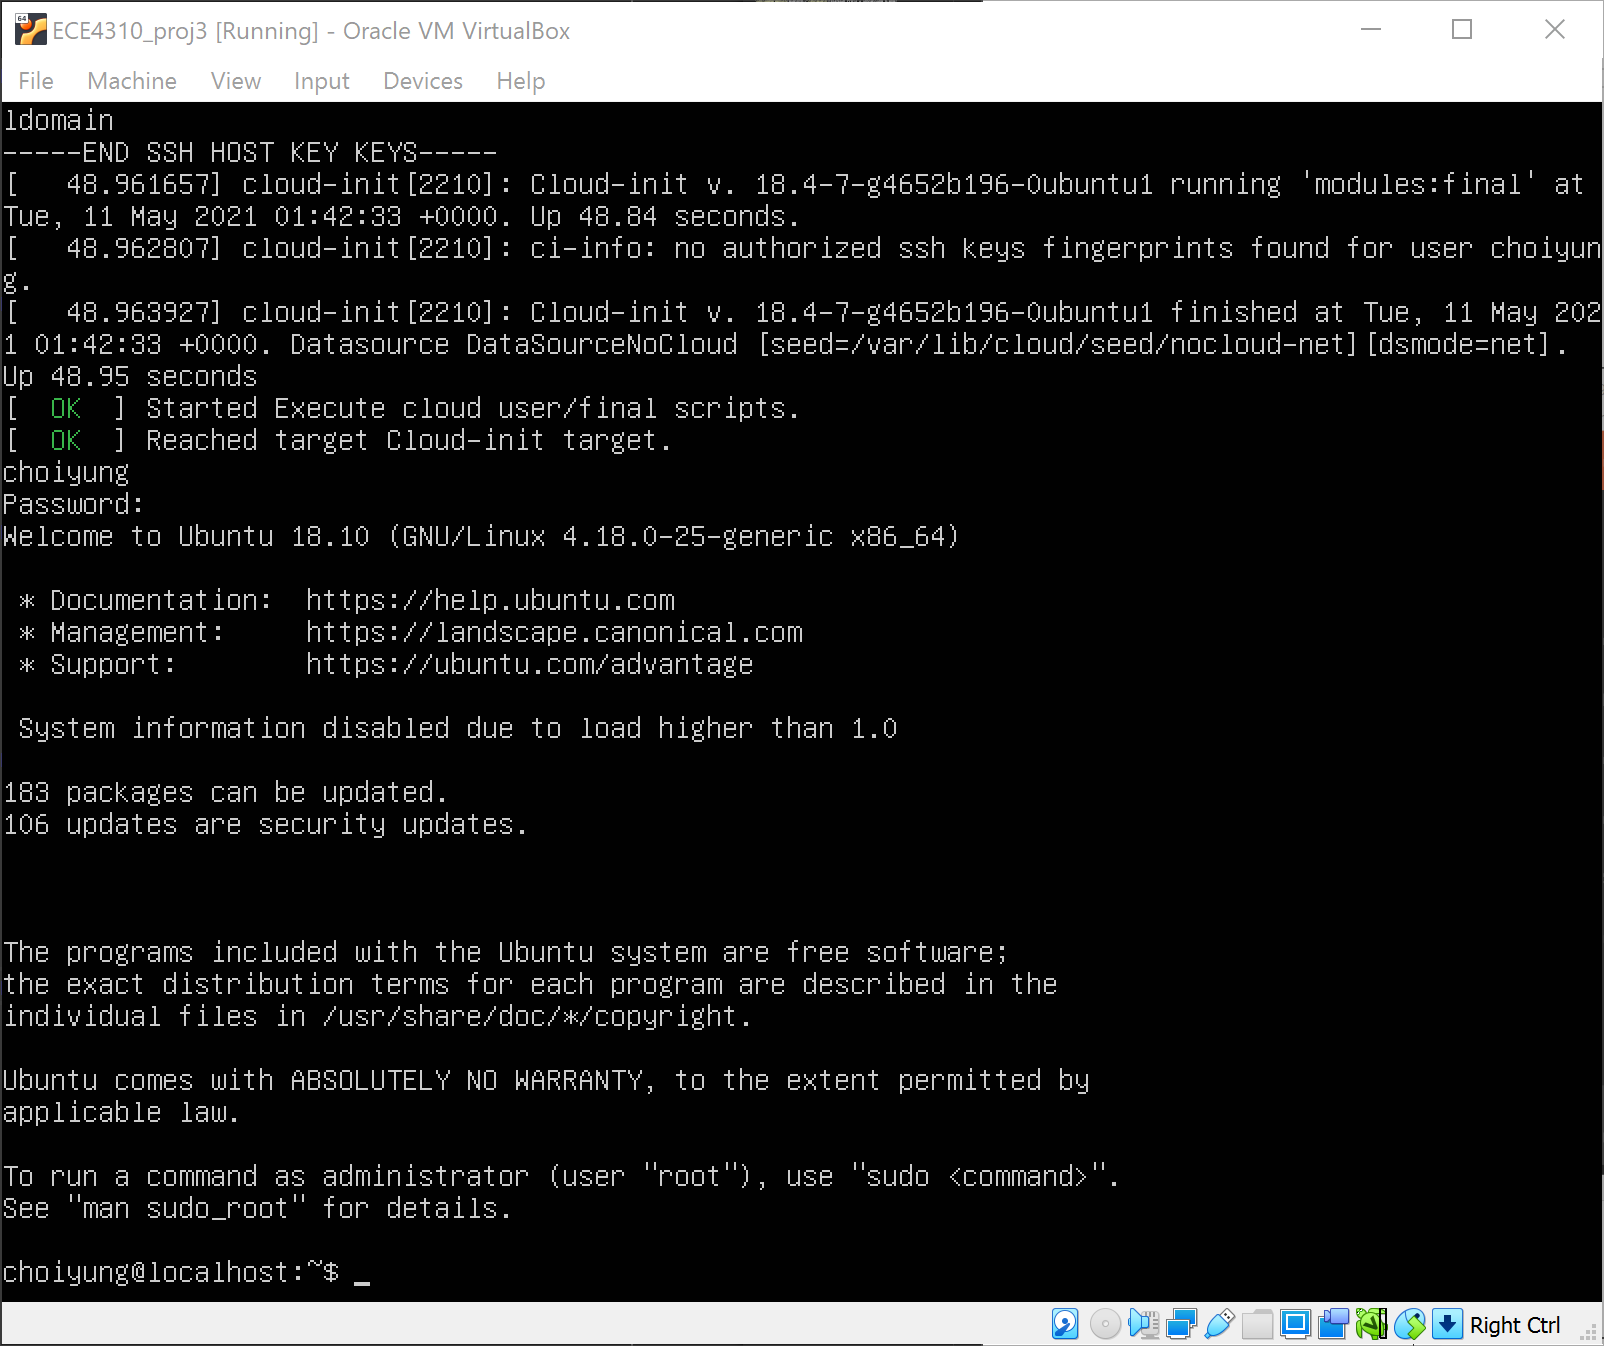
\includegraphics[width=0.7\textwidth]{ECE4310_Proj3_1_logged_in.png}
\end{figure}

\section{Virtual Machine Specifications}

\subsection{\texttt{cat /proc/cpuinfo}}

\begin{figure}[H]

  \caption{Output of \texttt{cat /proc/cpuinfo}}
  \centering
  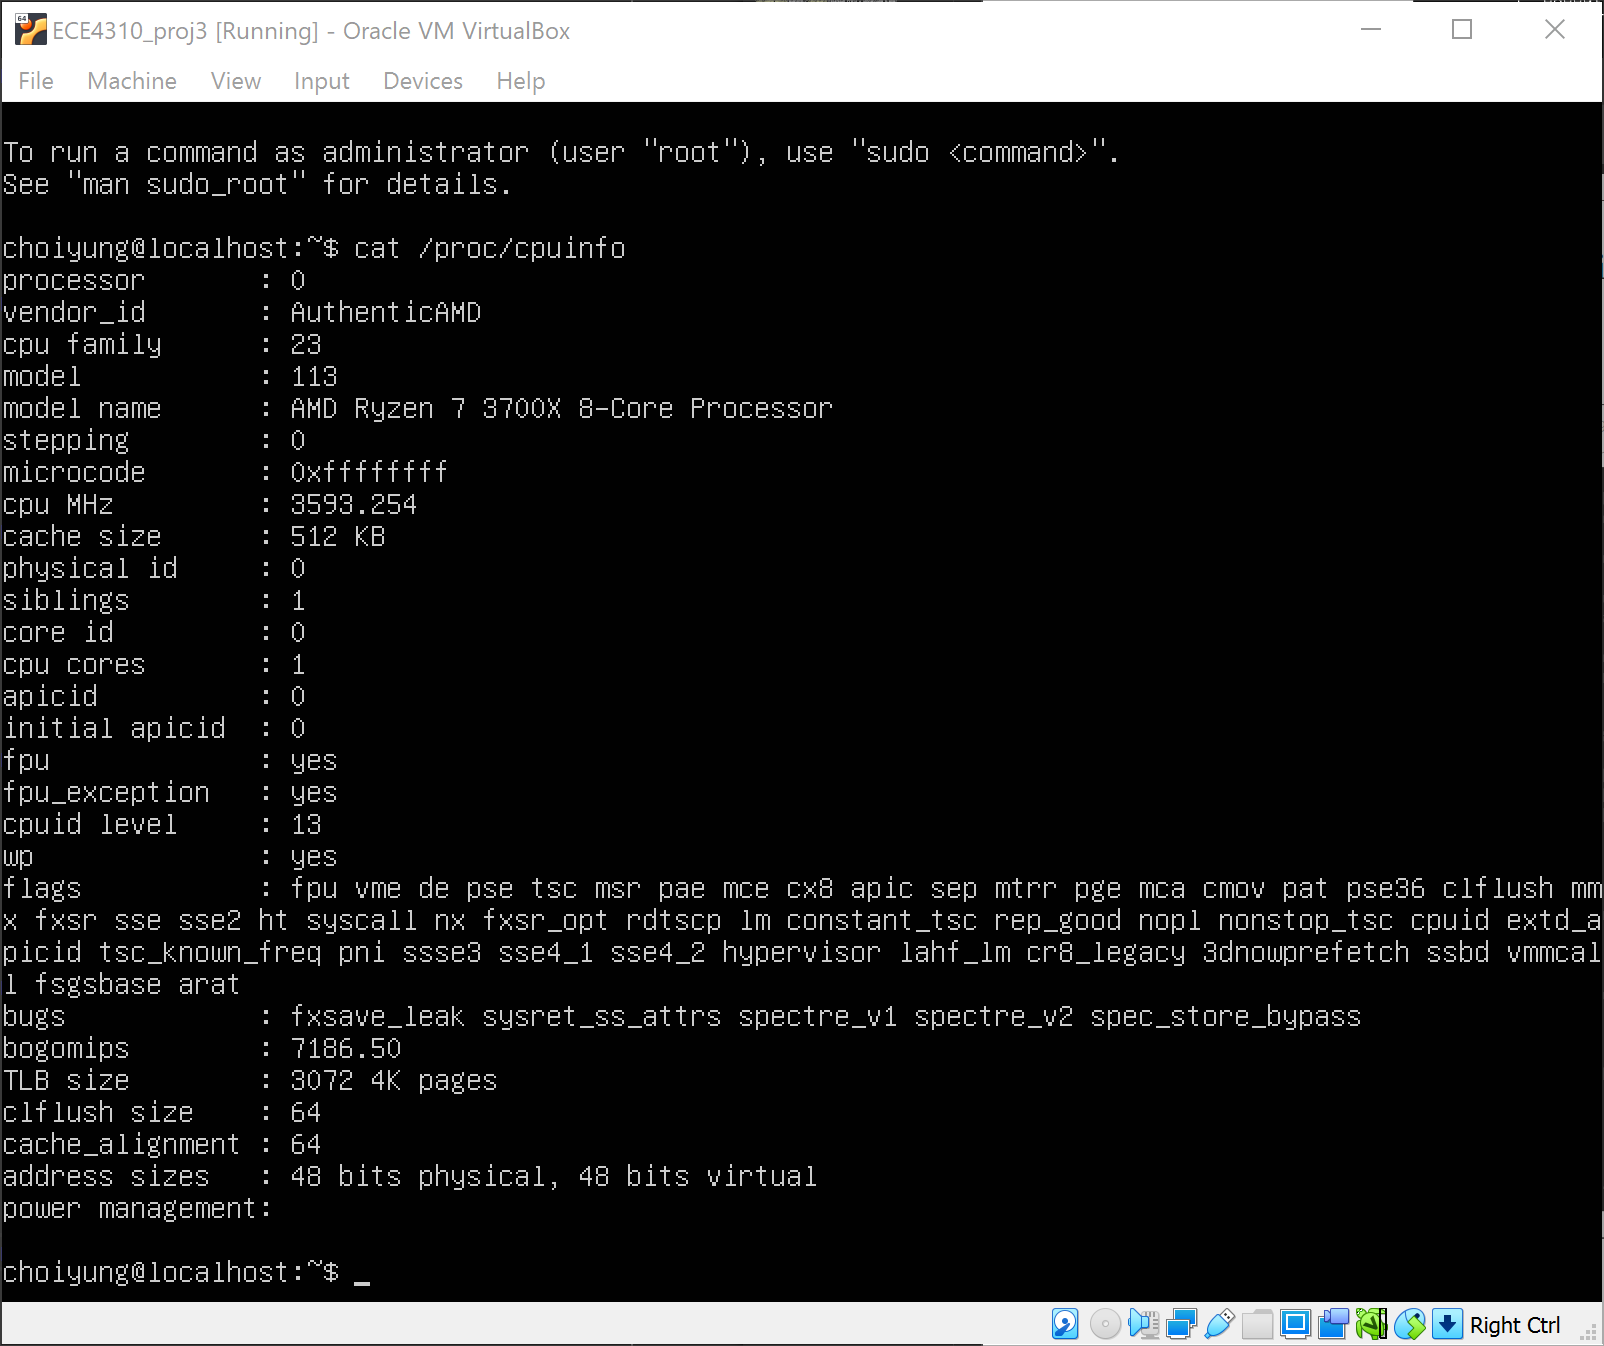
\includegraphics[width=0.59\textwidth]{ECE4310_Proj3_2_cpuinfo.png}
\end{figure}

1 CPU is assigned to my VM and it is an AMD Ryzen 7 3700X

\subsection{\texttt{cat free -m}}

\begin{figure}[H]

  \caption{Output of \texttt{free -m}}
  \centering
  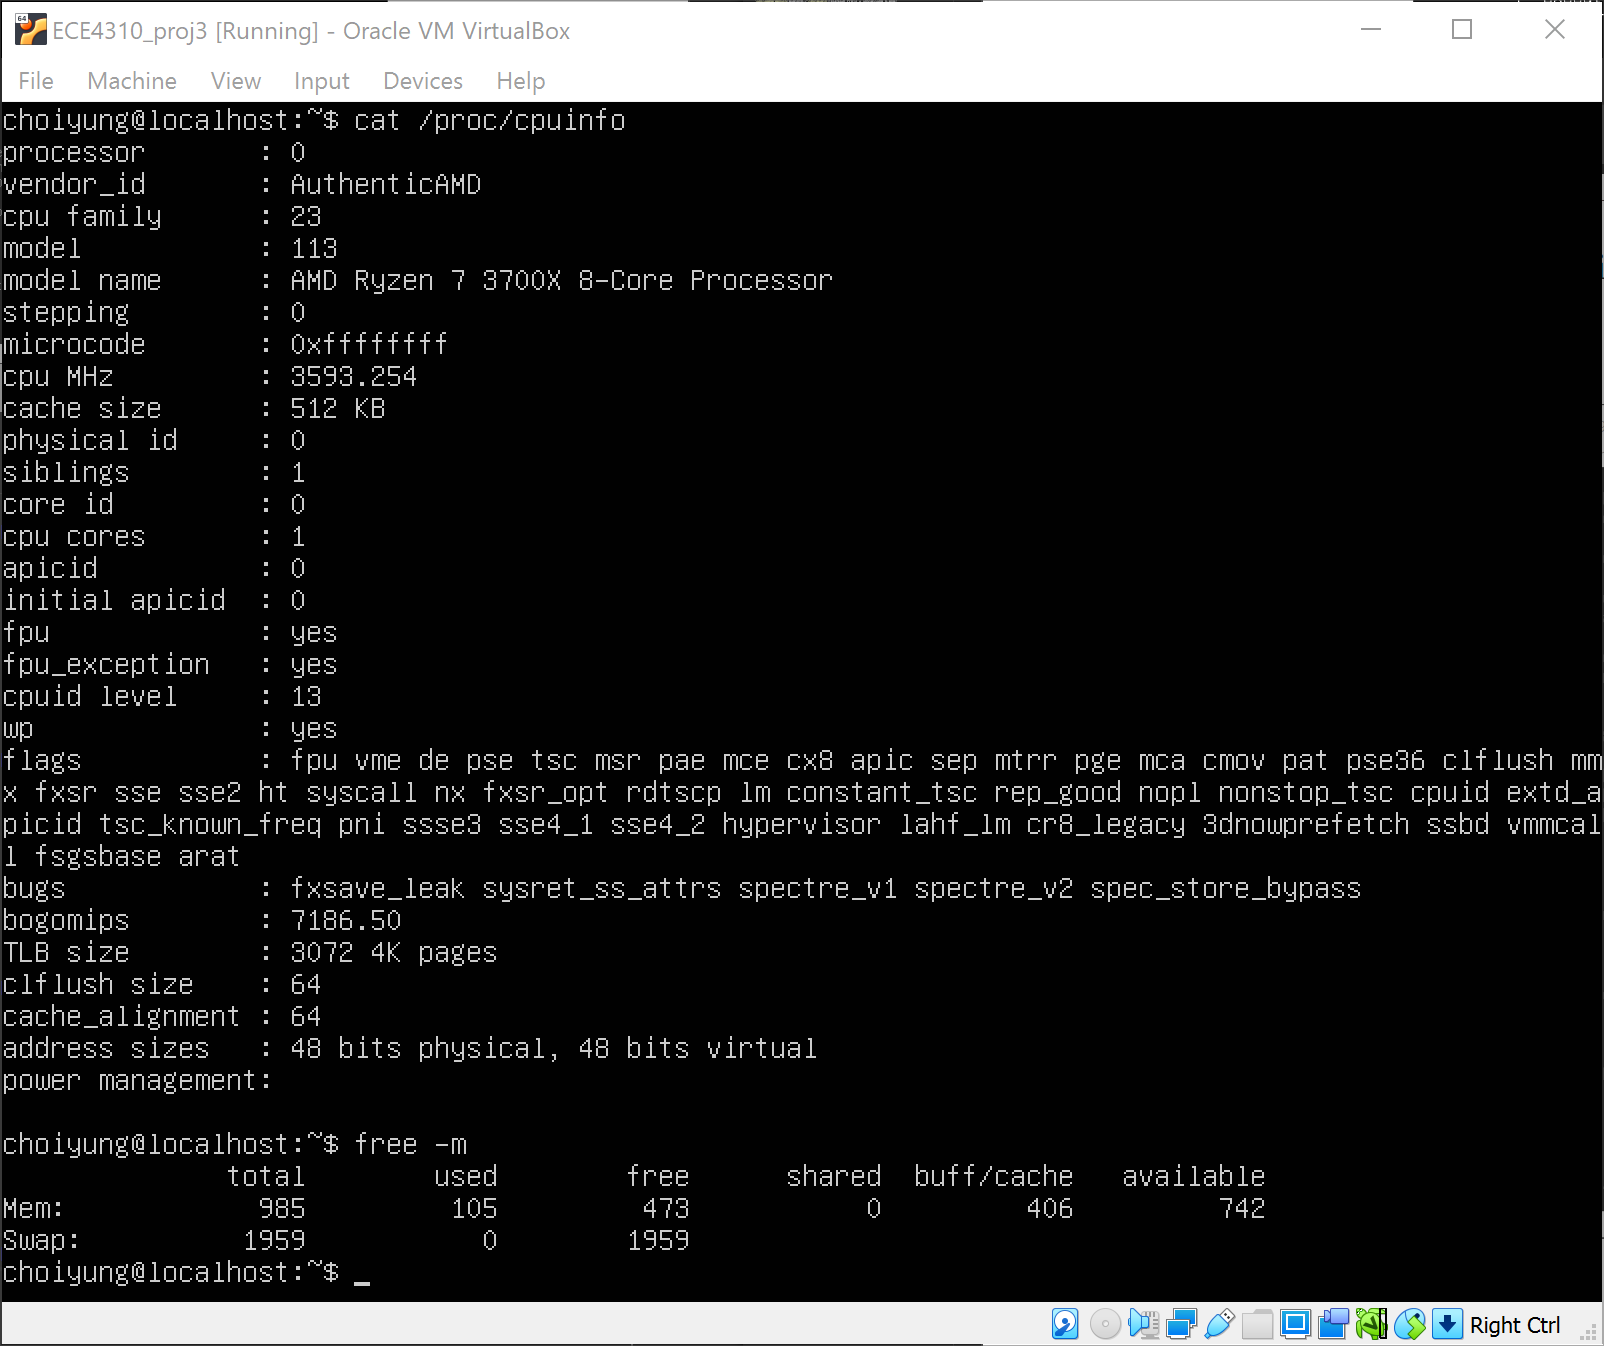
\includegraphics[width=0.59\textwidth]{ECE4310_Proj3_2_free.png}
\end{figure}

985 MB of memory is assigned to the VM

\subsection{\texttt{cat uname -a}}

\begin{figure}[H]

  \caption{Output of \texttt{uname -a}}
  \centering
  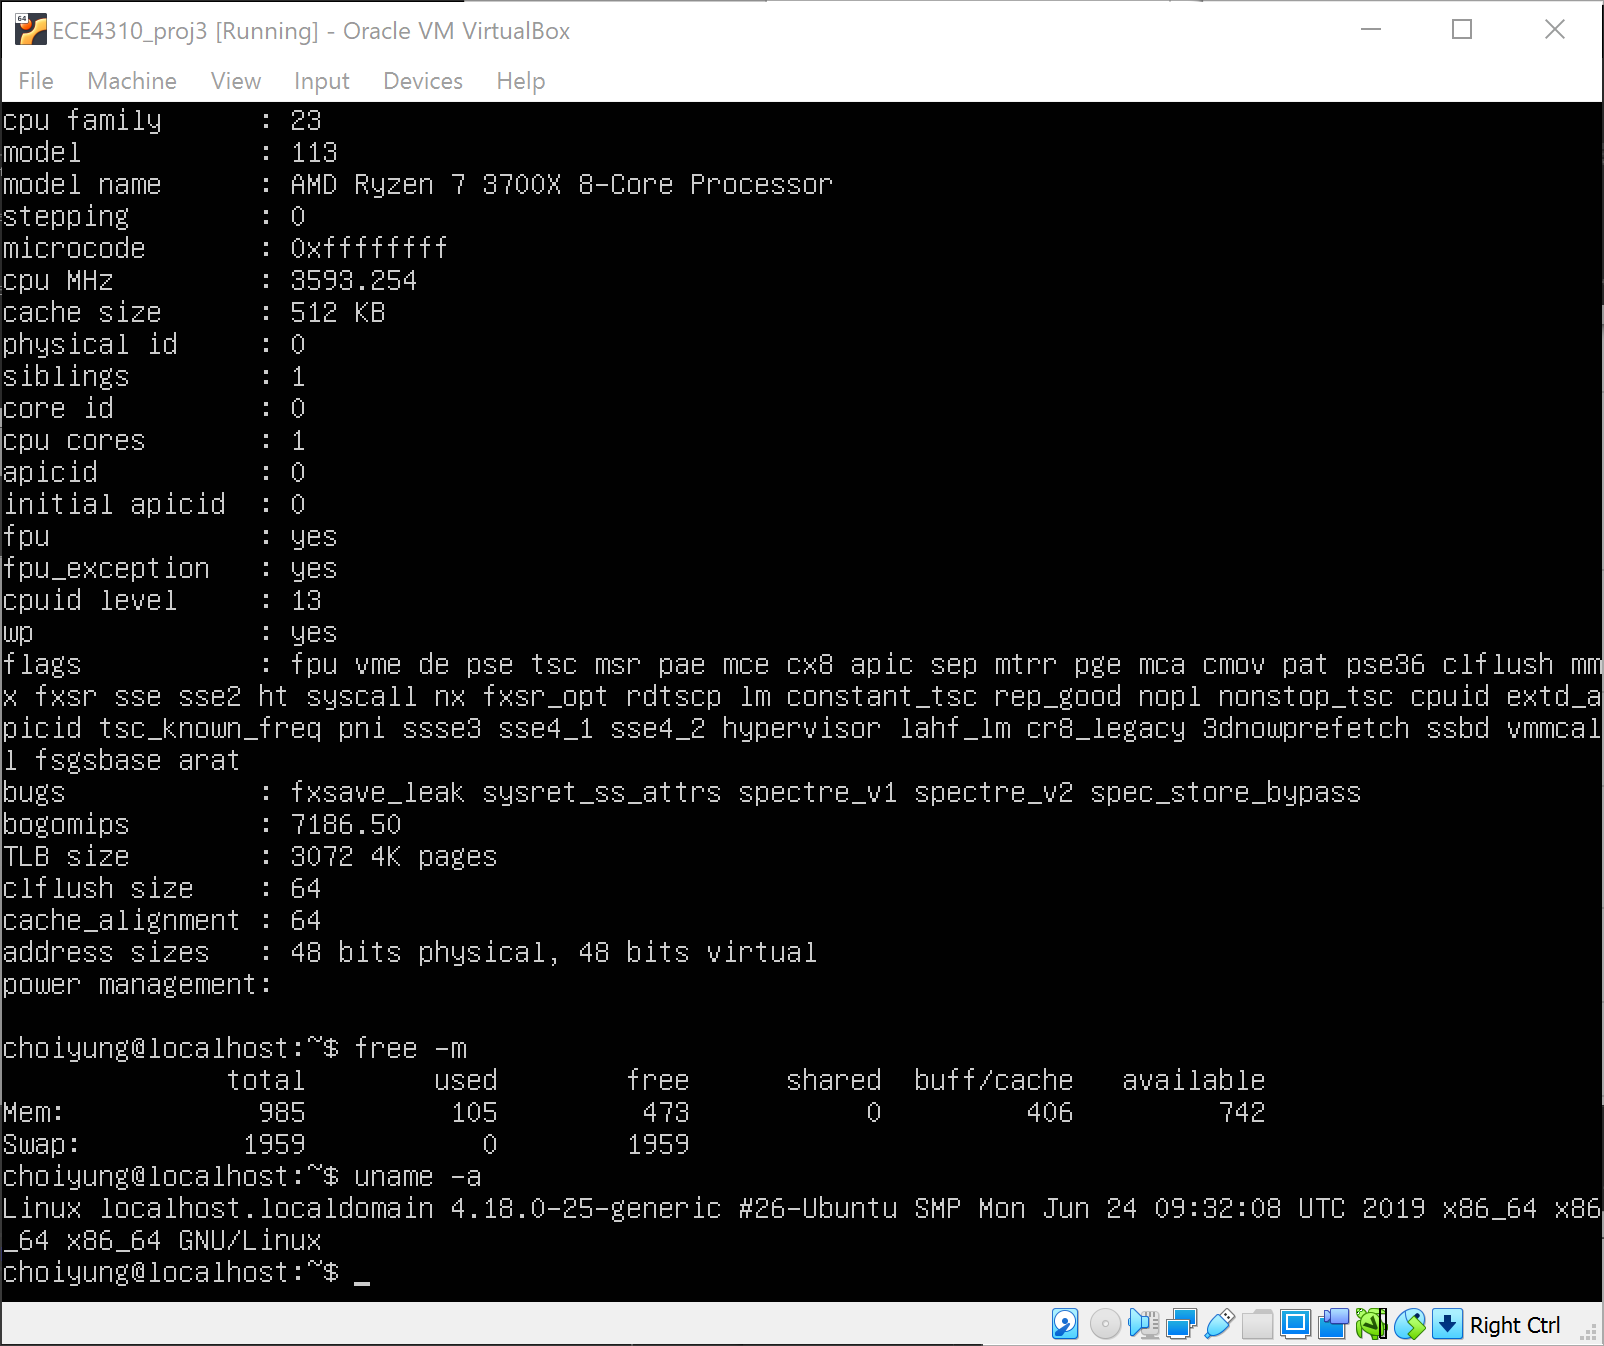
\includegraphics[width=0.59\textwidth]{ECE4310_Proj3_2_uname.png}
\end{figure}

The linux kernel version is 4.18.0-25-generic


\subsection{\texttt{sudo fdisk -l /dev/sda}}

\begin{figure}[H]

  \caption{Output of \texttt{sudo fdisk -l /dev/sda}}
  \centering
  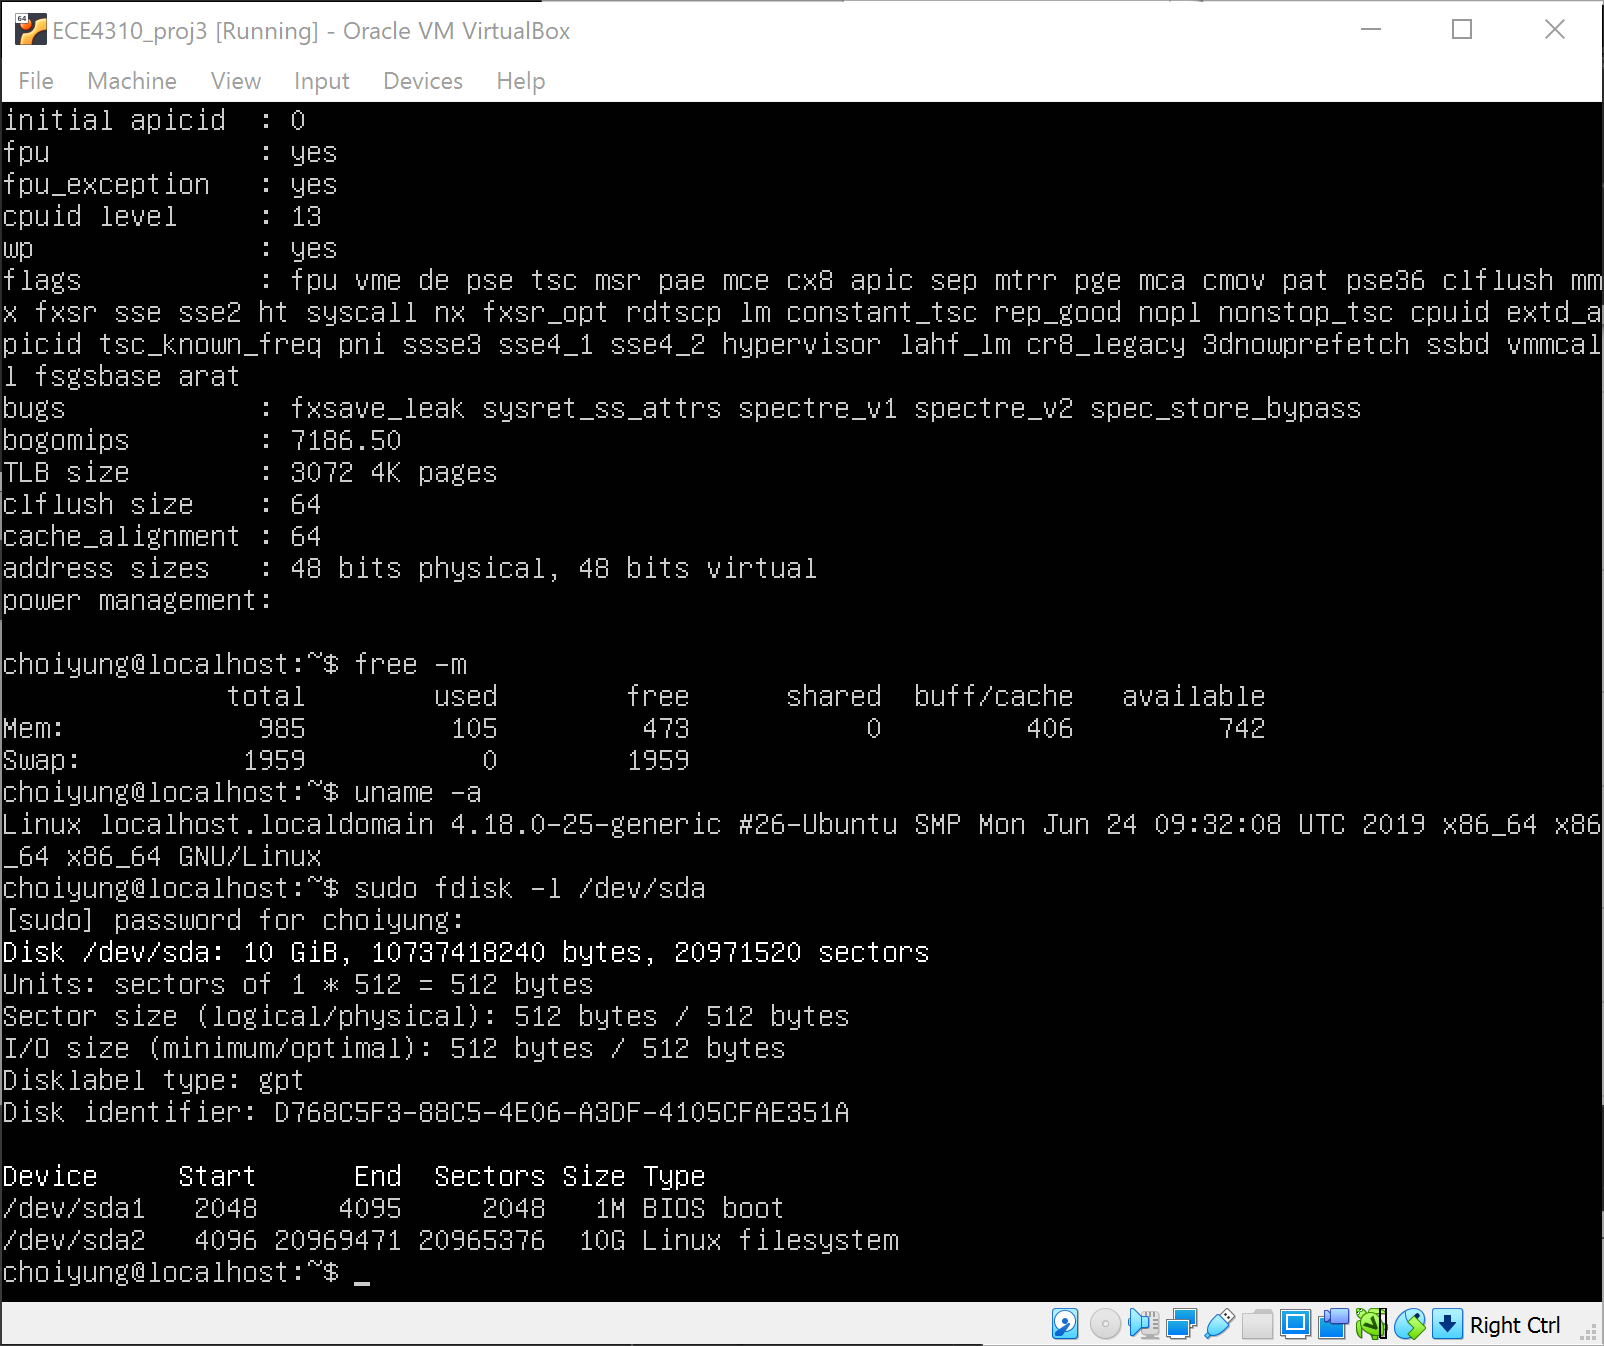
\includegraphics[width=0.59\textwidth]{ECE4310_Proj3_2_fdisk.png}
\end{figure}

10737418240 bytes $\approx$ 10 GB of disk space is allocated to the VM

\subsection{\texttt{lspci | grep Ether}}

\begin{figure}[H]

  \caption{Output of \texttt{lspci | grep Ether}}
  \centering
  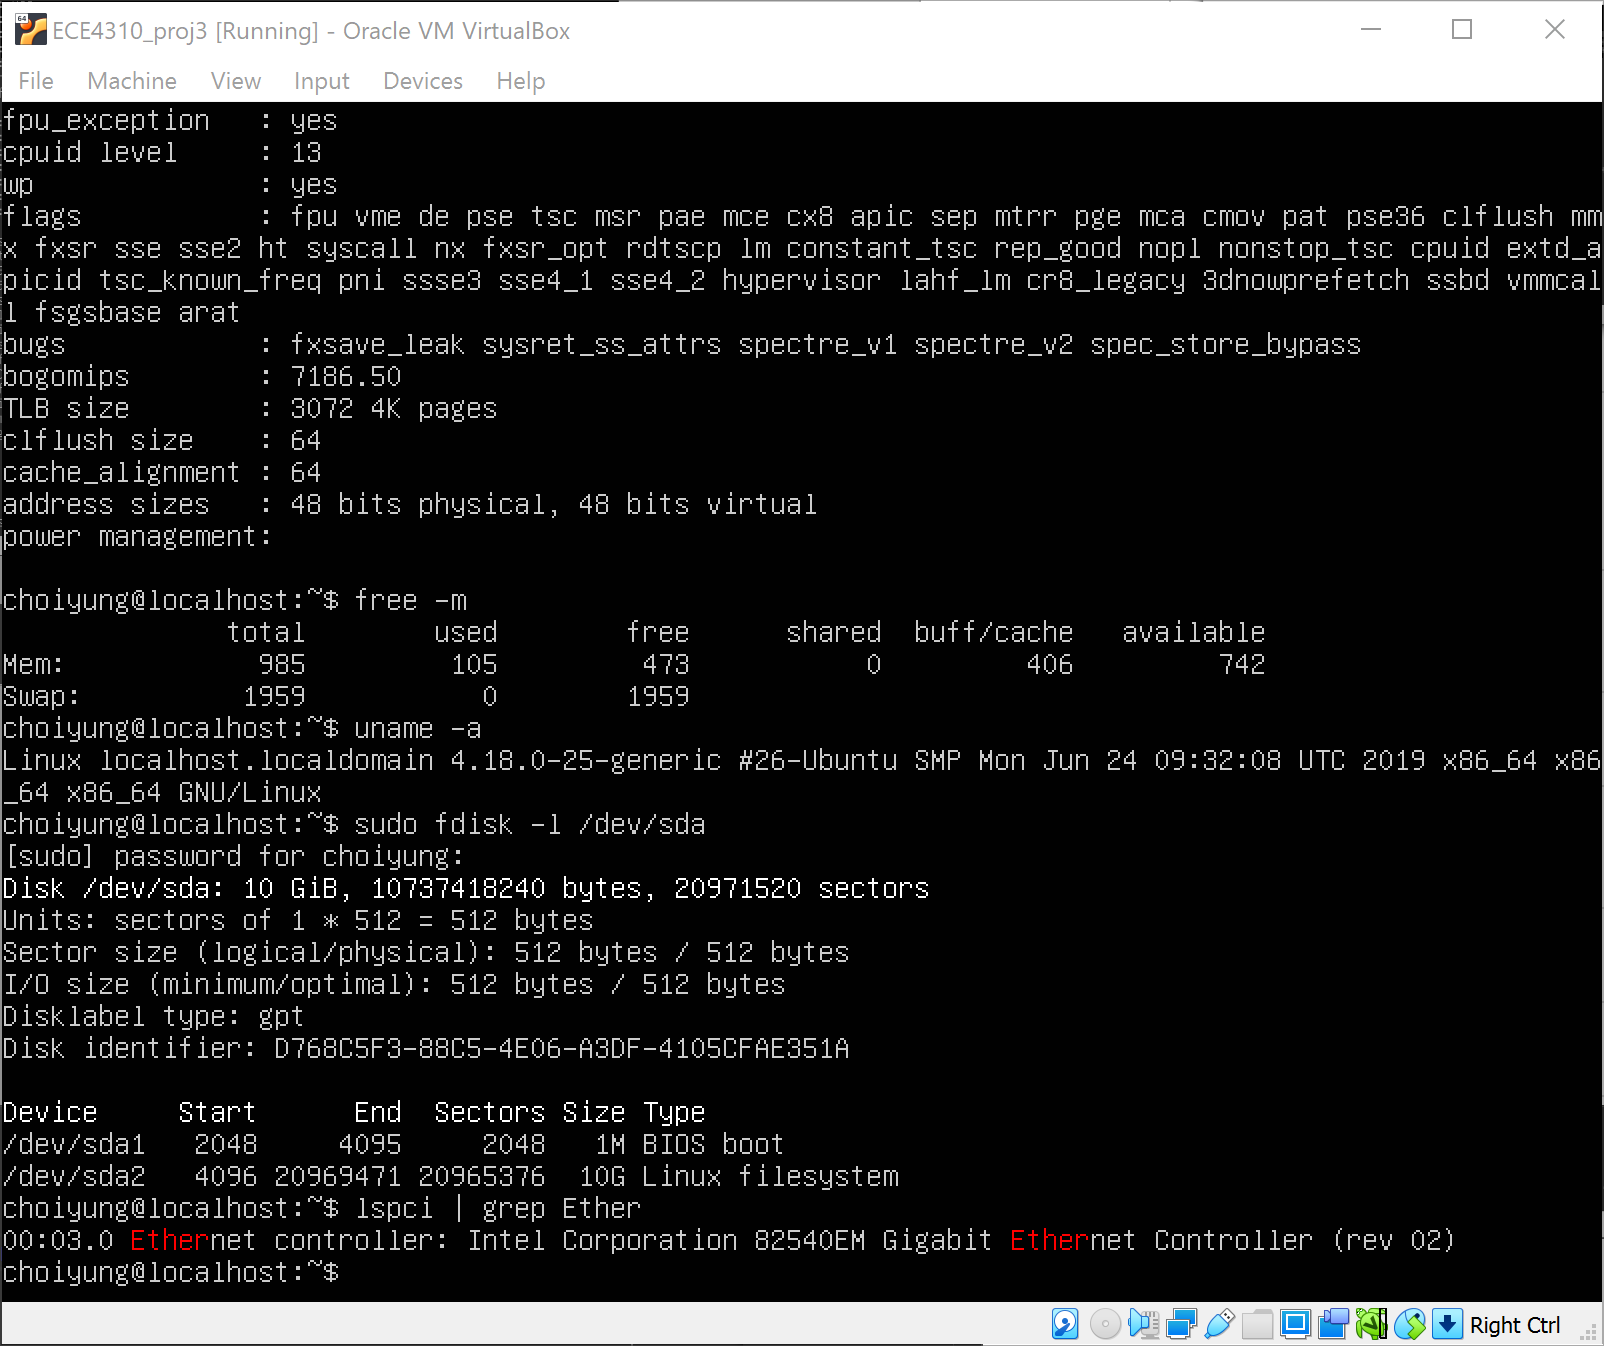
\includegraphics[width=0.59\textwidth]{ECE4310_Proj3_2_lspci.png}
\end{figure}

An Intel Corporation 82540EM Gigabit Ethernet Controller (rev 02) network card is installed.

\end{document}


% \section{\texttt{vmstat} and \texttt{free}}

% \subsection{\texttt{vmstat}}

% \begin{figure}[H]

%   \caption{Output of \texttt{vmstat}}
%   \centering
%   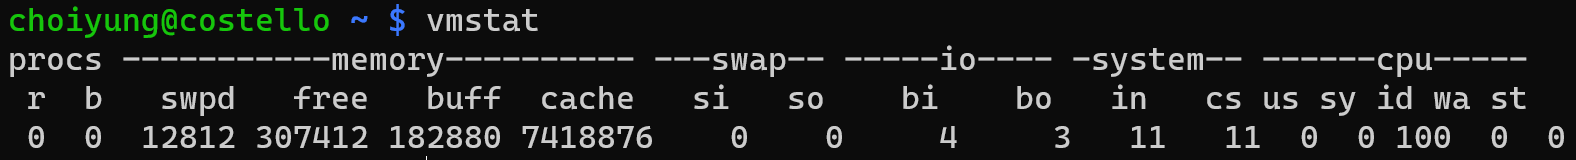
\includegraphics[width=0.7\textwidth]{ECE4310_proj2_vmstat.png}
% \end{figure}

% \begin{figure}[H]
%   \caption{Output of \texttt{man vmstat}}
%   \centering
%   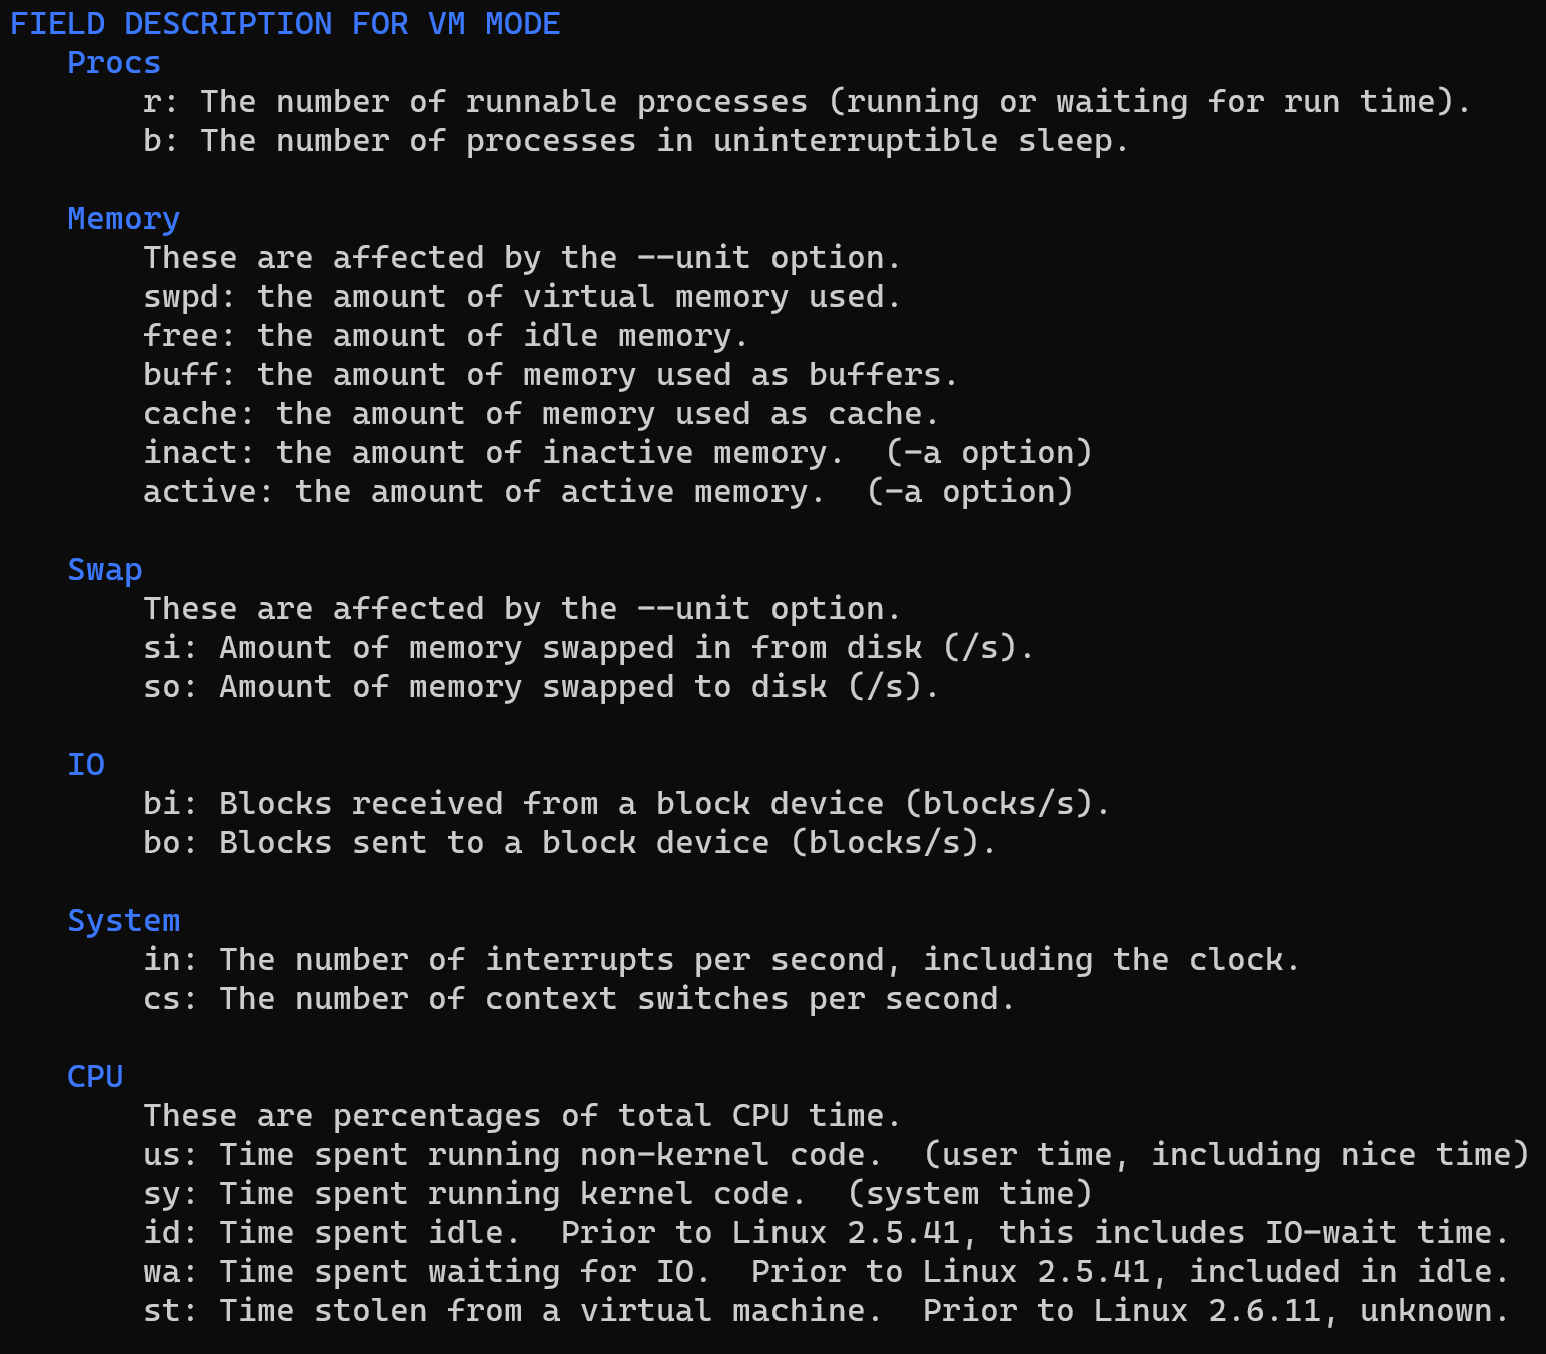
\includegraphics[width=0.7\textwidth]{ECE4310_proj2_vmstat_man.png}
% \end{figure}

% According to the \texttt{man} page:
% \begin{itemize}
%   \item r indicate there are currently no processes running or waiting;
%   \item b indicate there are currently no processes in uninterruptible sleep;
%   \item swpd is the amount of virtual memory/swap memory/pagefile/backing store used;
%   \item free is the amount of physical memory not in use;
%   \item buff is the amount of physical memory used as buffers;
%   \item cache is the amount of physical memory used as caches;
%   \item si is the amount of swapping/paging in per second, indicating if some page was swapped back to physical memory;
%   \item so is the amount of swapping/paging out per second, indicating if some page was swapped to disk to free frames;
%   \item bi is the amount of blocks received from a block device, i.e. input from some hardware devices
%   \item bo is the amount of blocks sent to a block device, i.e. output to some hardware devices
%   \item in is the number of interrupts per second
%   \item cs is the number of context switches per second
%   \item us is the percentage of CPU time running non-kernel code
%   \item sy is the percentage of CPU time running kernel code
%   \item id is the percentage of CPU time being idle
%   \item wa is the percentage of CPU time waiting for IO
%   \item st is the percentage of CPU time stolen from virtual machine
% \end{itemize}

% From the \texttt{vmstat} output, it can be determined that no user space processes are currently running or sleeping; 
% 12812B of backing store is in use; 307412B of physical memory is not in use; 182880B of physical memory is used as buffer; 
% 7418876B of physical memory is used as cache; There are no paging in or paging out, meaning there are enough physical memory for processes running;
% Some blocks are being transferred indicating accesses to block devices (usually mass storage); Multiple processes are running, hence the interrupts and context switching; 
% and CPU spent almost all its time being idle. 


% \subsection{\texttt{free}}

% \begin{figure}[H]

%   \caption{Output of \texttt{free}}
%   \centering
%   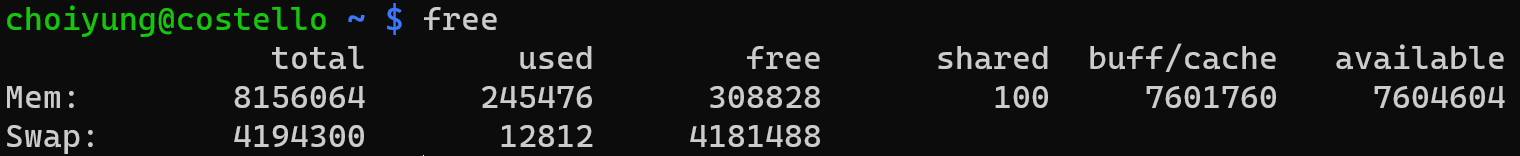
\includegraphics[width=0.7\textwidth]{ECE4310_proj2_free.png}
% \end{figure}

% \begin{figure}[H]
%   \caption{Output of \texttt{man free}}
%   \centering
%   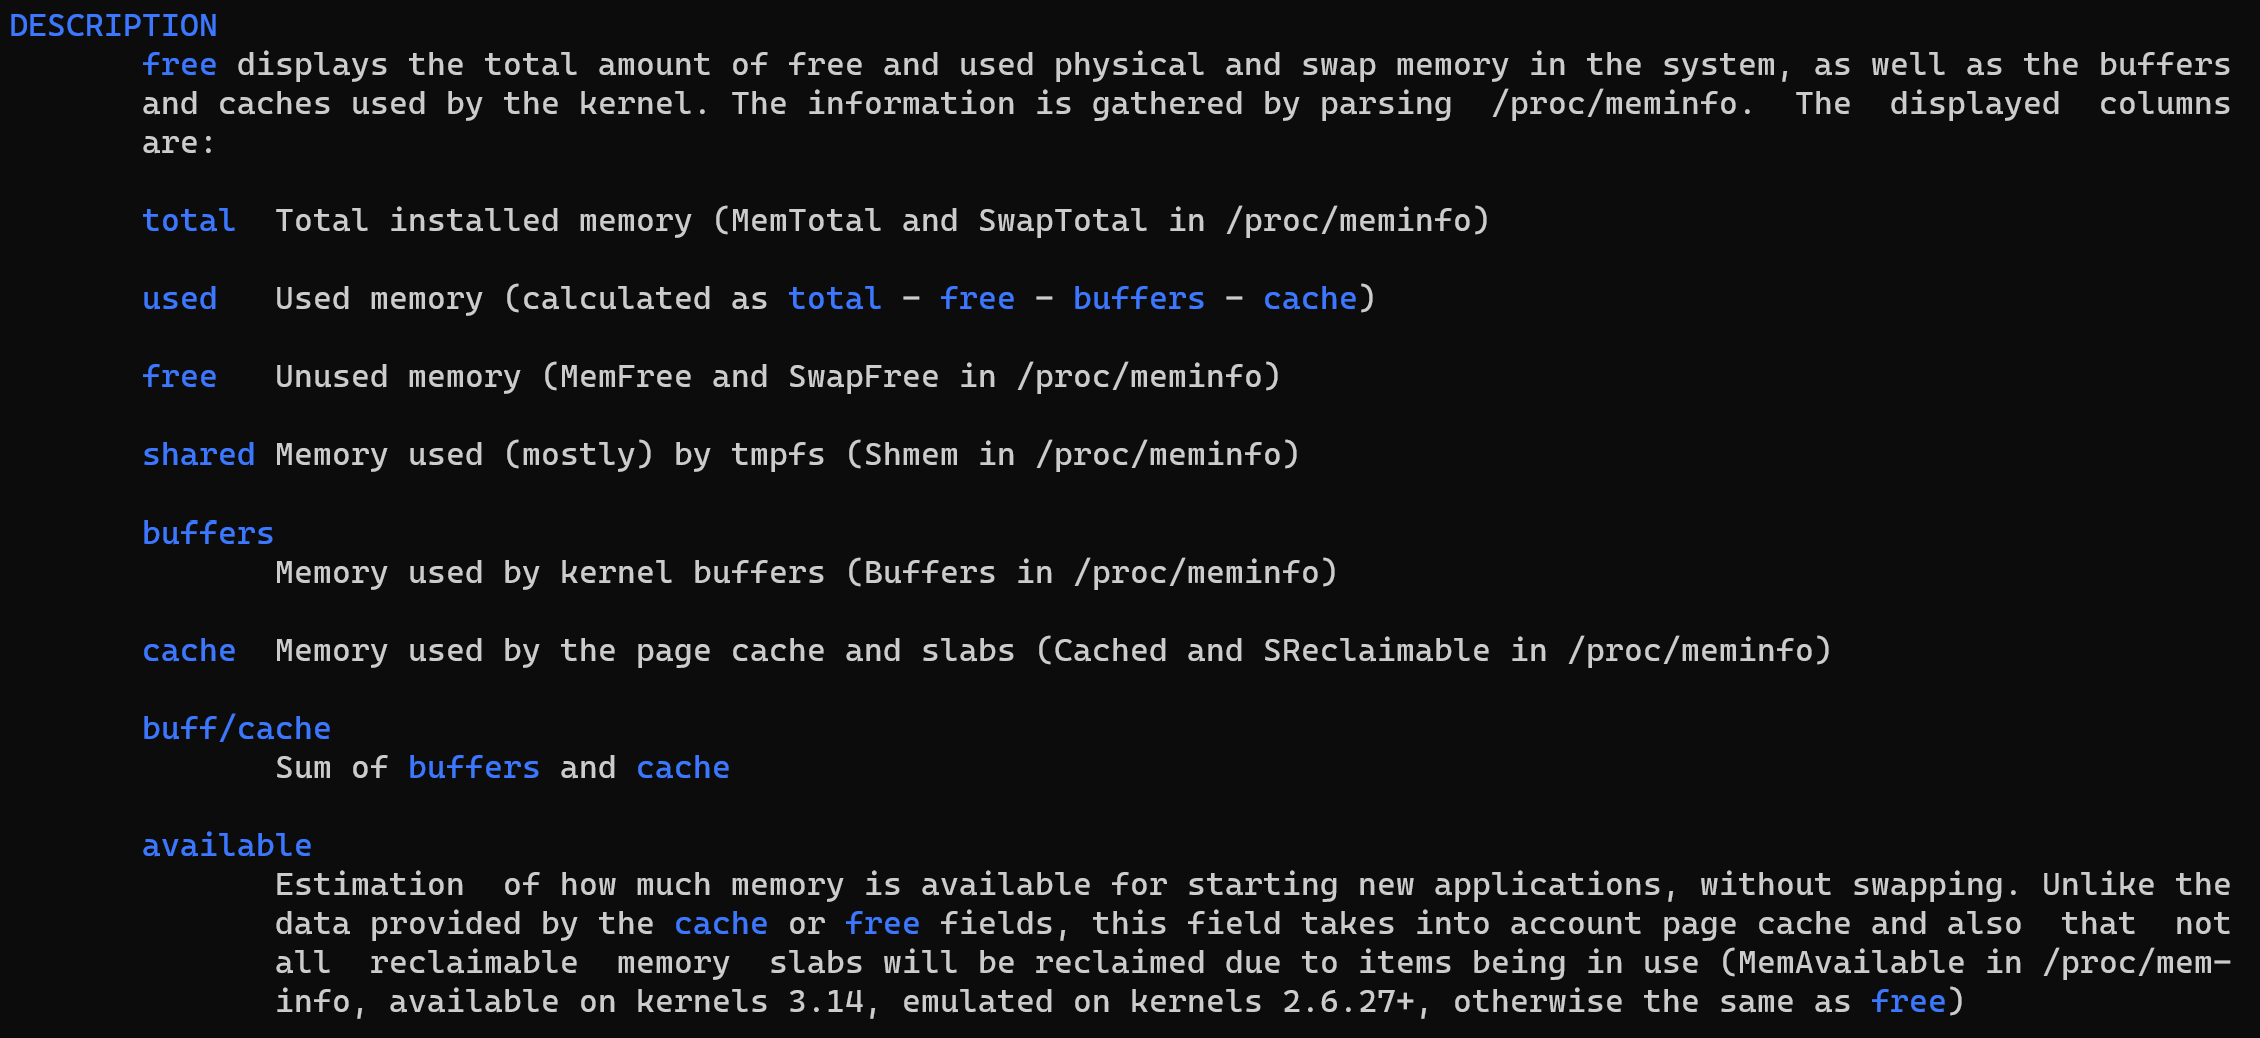
\includegraphics[width=0.7\textwidth]{ECE4310_proj2_free_man.png}
% \end{figure}

% From the \texttt{free} output, it can be determined that the system have a total of 8156064B of physical memory, 
% 245476B are allocated to processes, 308828B of physical memory are not used, 100B seems to be used mostly by tmpfs to provide a fast access file system, 
% 7601760B are used as buffers or cache, and 7604604B can be allocated to new process. 
% Also, there are a total of 4194300B of mass storage space allocated for backing store, 12812B of them are used and 4181488B are not.

% \section{Paging Simulation}
% \subsection*{Code}
% \lstinputlisting[language=C]{ECE4310_proj2_2.c}
% \begin{figure}[H]

%   \caption{Output of the code}
%   \centering
%   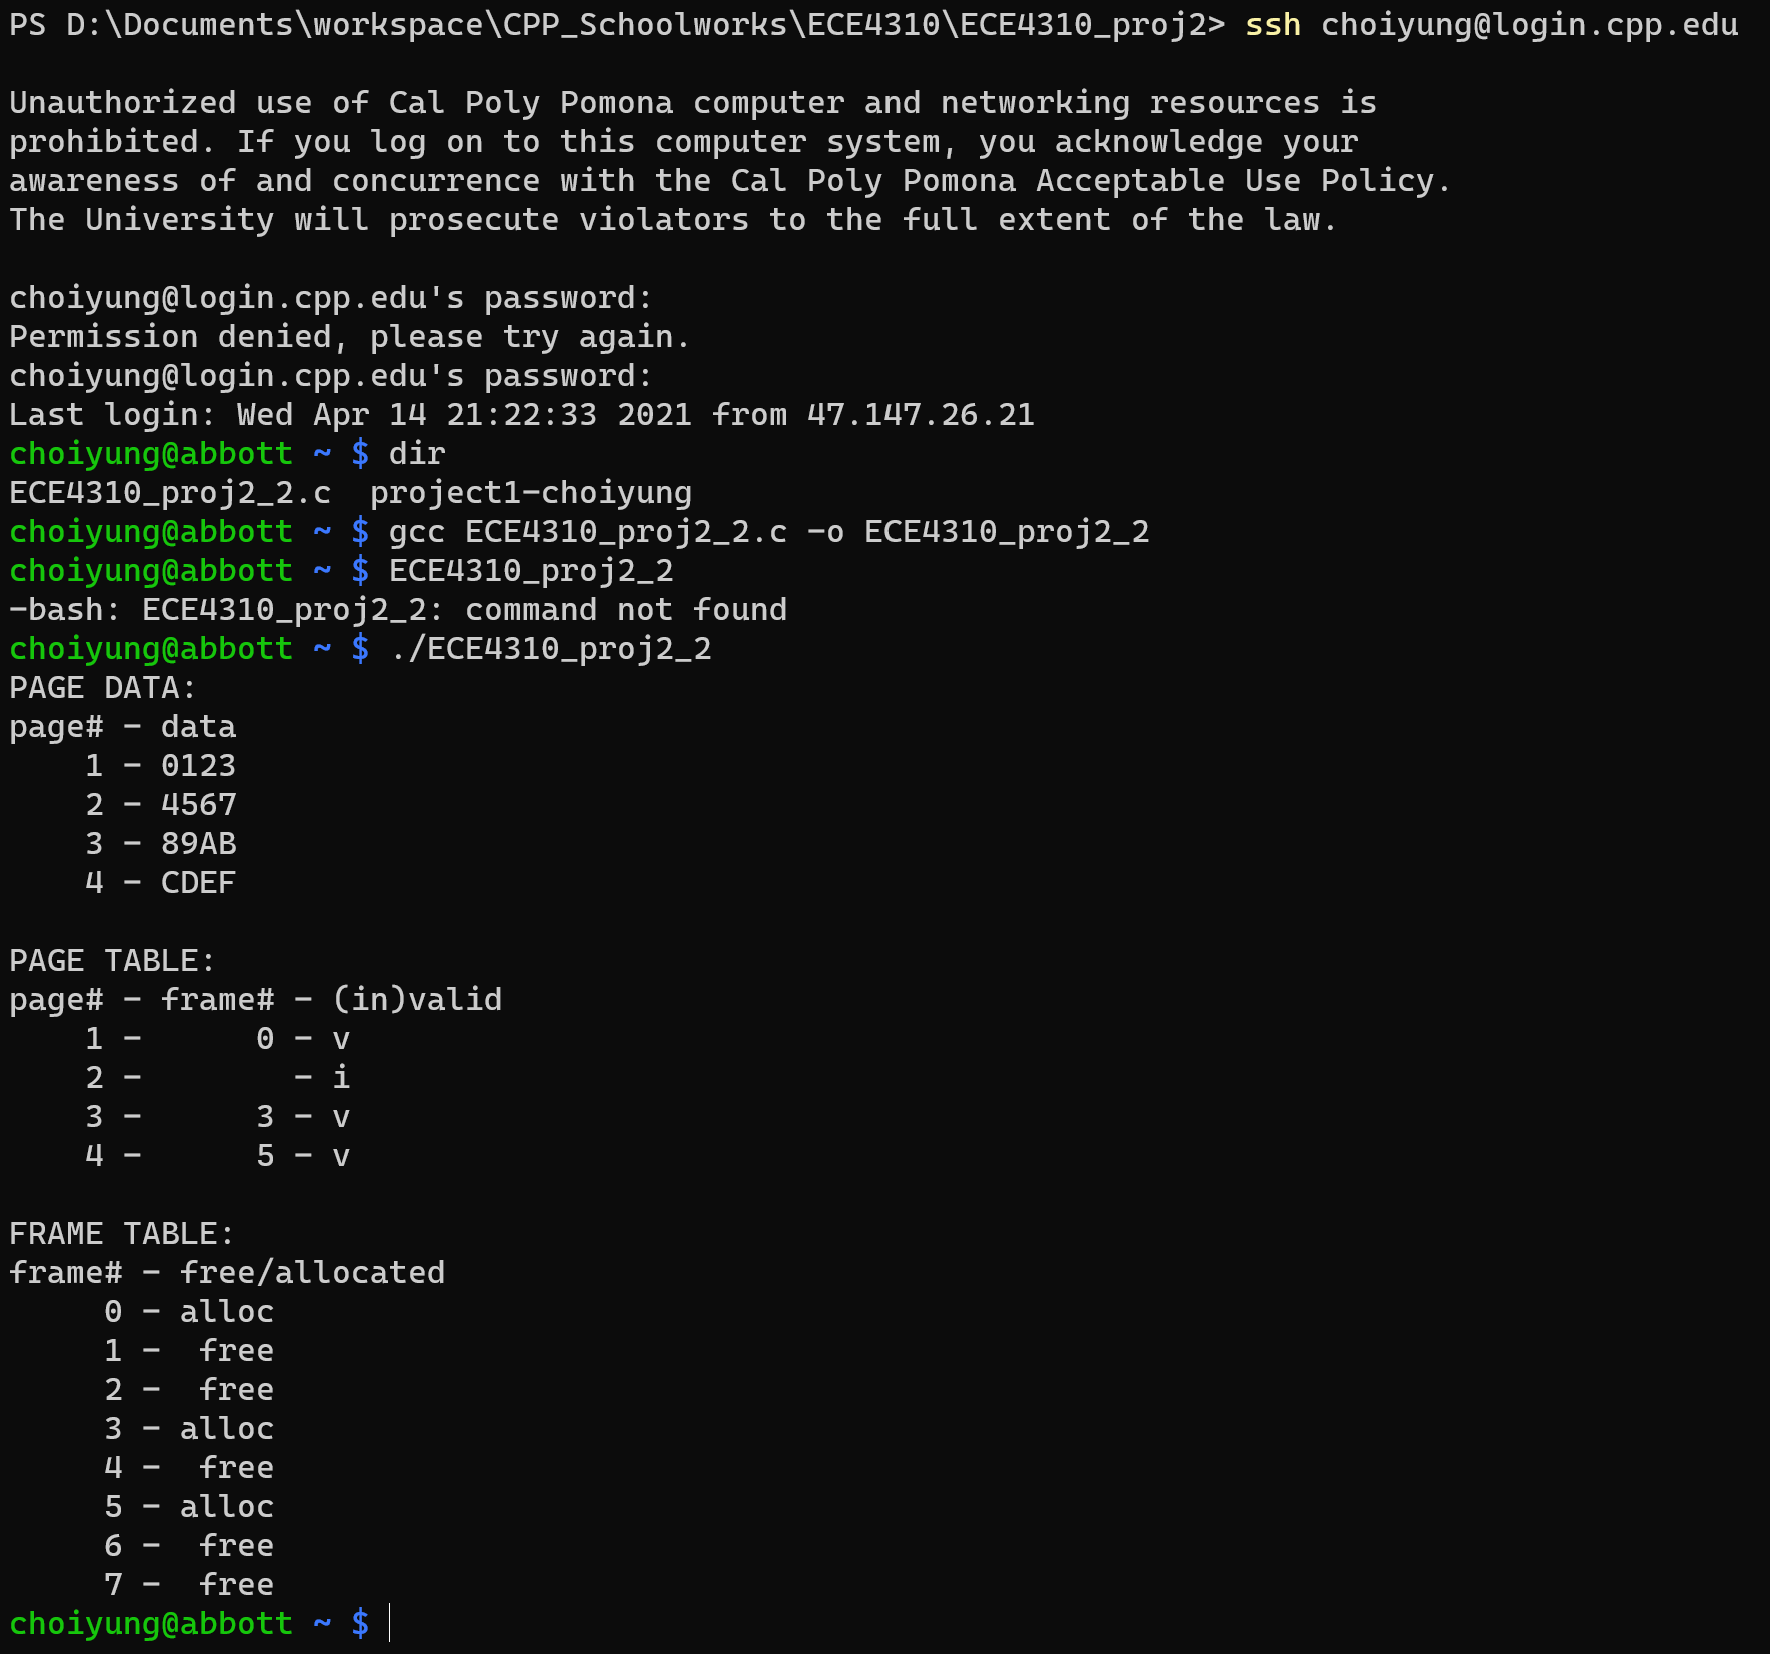
\includegraphics[width=0.7\textwidth]{ECE4310_proj2_2_abbott.png}
% \end{figure}

